\chapter{Determination of the Strong Coupling Constant}
\label{chap:Alphas}
The inclusive jet production cross-section at hadron colliders mainly depends on the strong coupling constant \alps for a given centre-of-mass energy. Hence the measurements of the inclusive jet cross-section and jet properties provide a direct probe to measure the strong coupling constant. The measurement of \alps has been already done by various experiments such as CMS~\cite{Chatrchyan:2013txa, Chatrchyan:2013haa, Khachatryan:2014waa, CMS:2014mna, Khachatryan:2016mlc}, ATLAS~\cite{ATLAS:2015yaa}, D0~\cite{Abazov:2009nc, Abazov:2012lua}, H1~\cite{Andreev:2014wwa, Andreev:2016tgi}, and ZEUS~\cite{Abramowicz:2012jz}. In this thesis, the measurements of differential inclusive 2-jet and 3-jet event cross-sections as well as the cross-section ratio \ratio, as a function of \httwo are used to extract the value of the strong coupling constant at  the  scale  of  the  Z boson mass \alpsmz. The differential inclusive jet production cross-section upto at NLO is given by \cite{Affolder:2001hn} :

 \begin{equation}
 \frac{d\sigma}{d(\httwo)} = \alpha_S^2(\mur)\hat{X}^{(0)}(\muf,\httwo)\big[1~\plus \alpha_S(\mur)K1(\mur, \muf,\httwo)\big]
 \label{eqn:SigmaNLO}
 \end{equation}

 where $\frac{d\sigma}{d(\httwo)}$ is the differential inclusive jet production cross-section as a function of \httwo, \mur and \muf are the renormalization and factorization scales set equal to \httwo, $\alpha_S^2(\mur)\hat{X}^{(0)}(\muf,\httwo)$ is the leading order (LO) contribution to the differential inclusive jet production cross-section and $\alpha_S^3(\mur)\hat{X}^{(0)}(\muf,\httwo)K1(\mur, \muf,\httwo)$ is the next-to-leading order (NLO) contribution. Equation~\ref{eqn:SigmaNLO} shows how the inclusive jet production cross-section varies with $\alpha_S(\mur)$. 
 
\section{Sensitivity of Measurements to \texorpdfstring{\alpsmz}{alpha-S(M(Z))}}
\label{sec:sensitivity}
 
For a fixed choice of \mur and \muf, different input values of \alpsmz to a PDF set will lead to different theory predictions of the differential cross-section distribution. This will give an estimate of the sensitivity of the theory predictions to the varying input value of \alpsmz. A comparison of the measured spectrum with the theory predictions obtained using all \alpsmz inputs will give a hint of the input value of \alpsmz for which the theory distribution has the closest matching with data. In this section, the sensitivity of the inclusive differential jet event cross-sections and cross-section ratio, \ratio to varying input values of \alpsmz for different PDF sets is demonstrated by plotting the ratios of data over theory predictions with central value of \alpsmz.

Figures~\ref{fig:sensitivity_2},~\ref{fig:sensitivity_3} and~\ref{fig:sensitivity_double_ratio} present the ratio of data to the theory predictions, corrected for NP effects, for all variations in \alpsmz available for the PDF sets CT10, CT14, MSTW2008, MMHT2014 and NNPDF2.3 at NLO evolution order as specified in Table~\ref{tab:nlopdfsets}, for inclusive 2-jet event cross-sections, inclusive 3-jet events cross-sections and ratio \ratio respectively. The \alpsmz value is varied in the range 0.112-0.127, 0.111-123, 0.110-0.130, 0.108-0.128 and 0.114-0.124 in steps of 0.001 for the CT10, CT14, MSTW2008, MMHT2014 and NNPDF2.3PDF sets, respectively. The error bars correspond to the total experimental uncertainty derived as quadratic sum from all uncertainty sources. The theory predictions are also corrected for EW effects for inclusive 2-jet events cross-section. A small slope increasing with \httwo is visible for most PDFs in both cross-sections. This effect is largely cancelled in the cross-section ratio. \ratio exhibits a flat behaviour with respect to the predictions for all five PDF sets in the whole range of \httwo up to 1680 GeV. Therefore, these data can be used to determine the strong coupling constant, although only up to 1 TeV for the cross-sections as long as electroweak corrections are not taken into account.

Moreover, the different sensitivity to \alpsmz caused by the leading power in \alps in the expansion of the 2-jet inclusive ($\propto\alps^2$) and the 3-jet inclusive cross-section ($\propto\alps^3$), and their ratio ($\propto\alps^1$) is clearly visible from the spread between the calculations for the smallest and largest value of \alpsmz within the same PDF set when passing through Figures~\ref{fig:sensitivity_2}--\ref{fig:sensitivity_double_ratio}.  This also demonstrates the potential of ratios $R_{mn}$ with $m$-$n$ \gr 1.

\begin{figure}[!htbp]
 \begin{center}
 \hspace*{-5mm}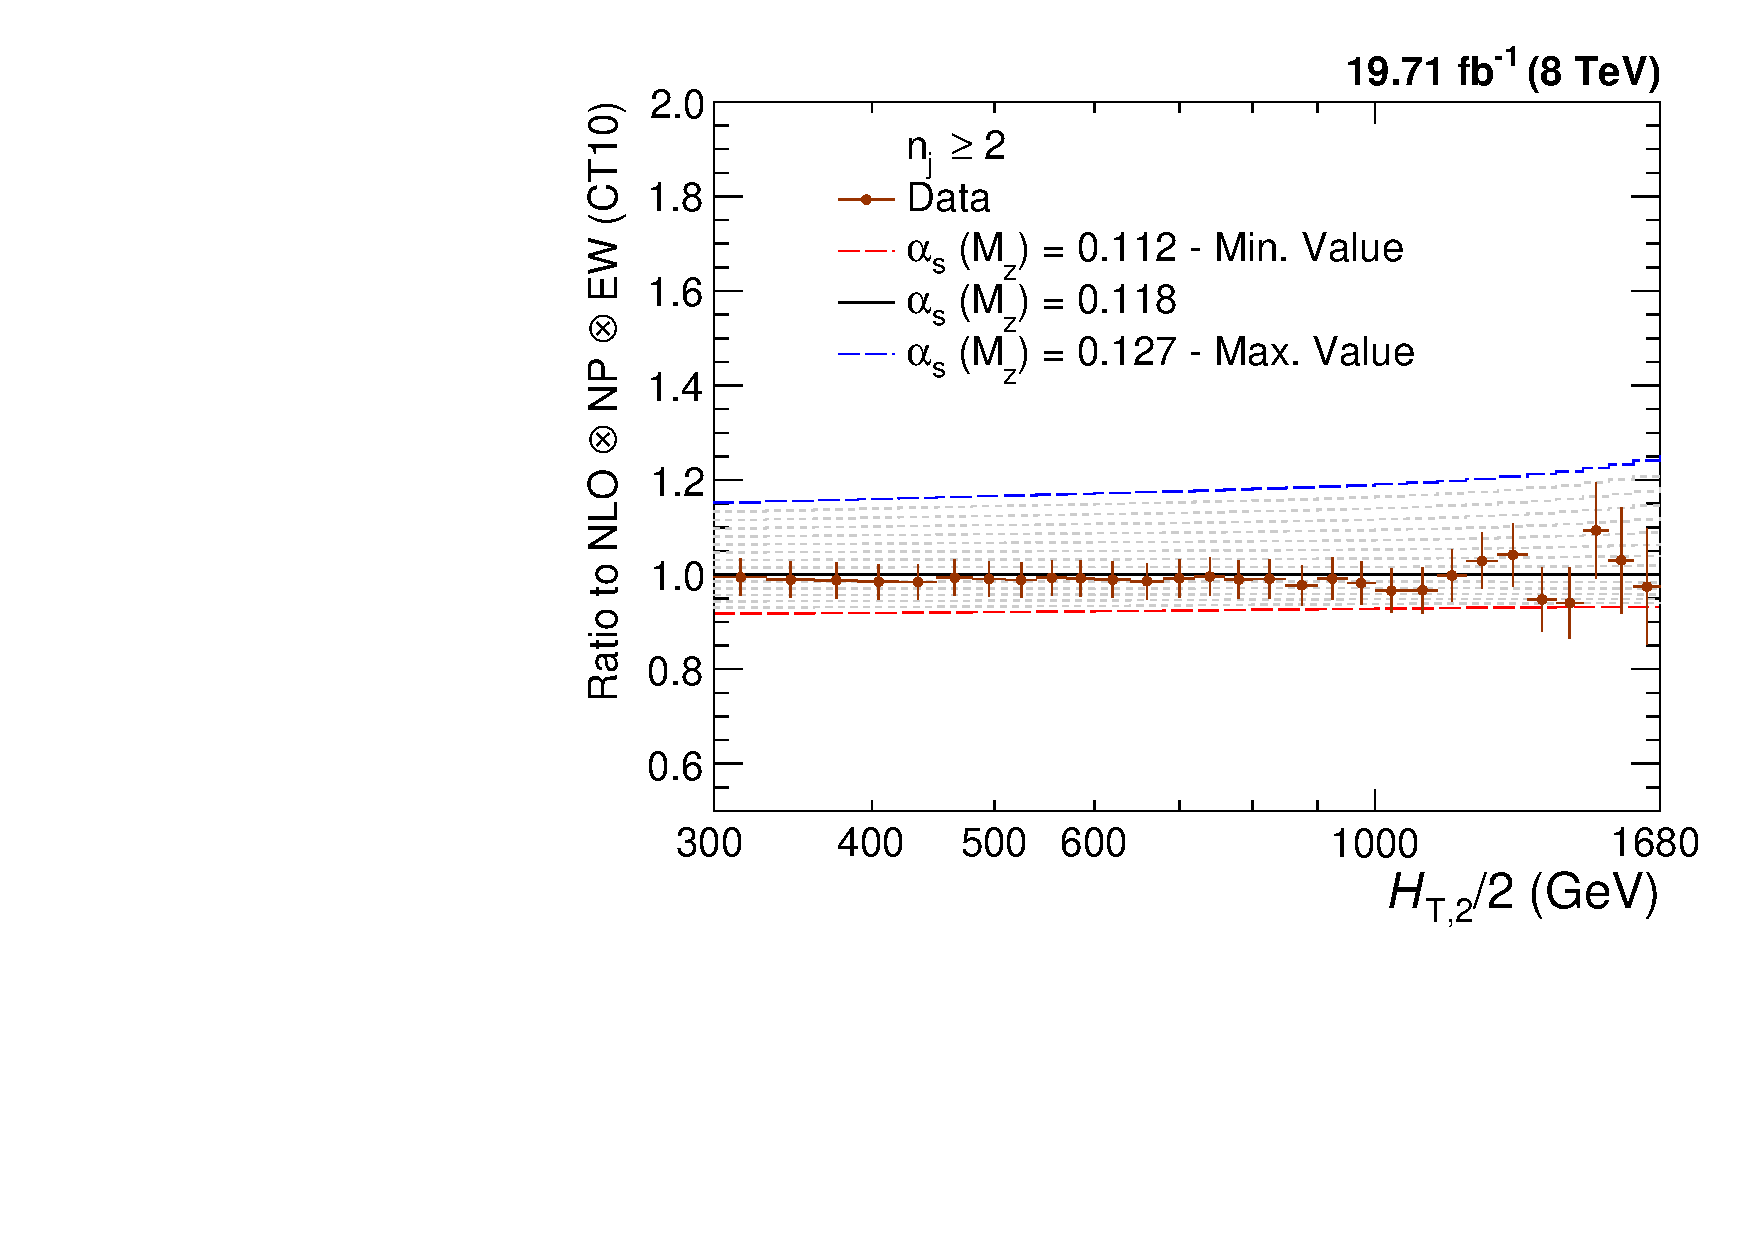
\includegraphics[width=0.51\textwidth]{Plots_HT_2_150/Sensitivity_2_ratio_NLO_CT10_EW.pdf}%
 ~~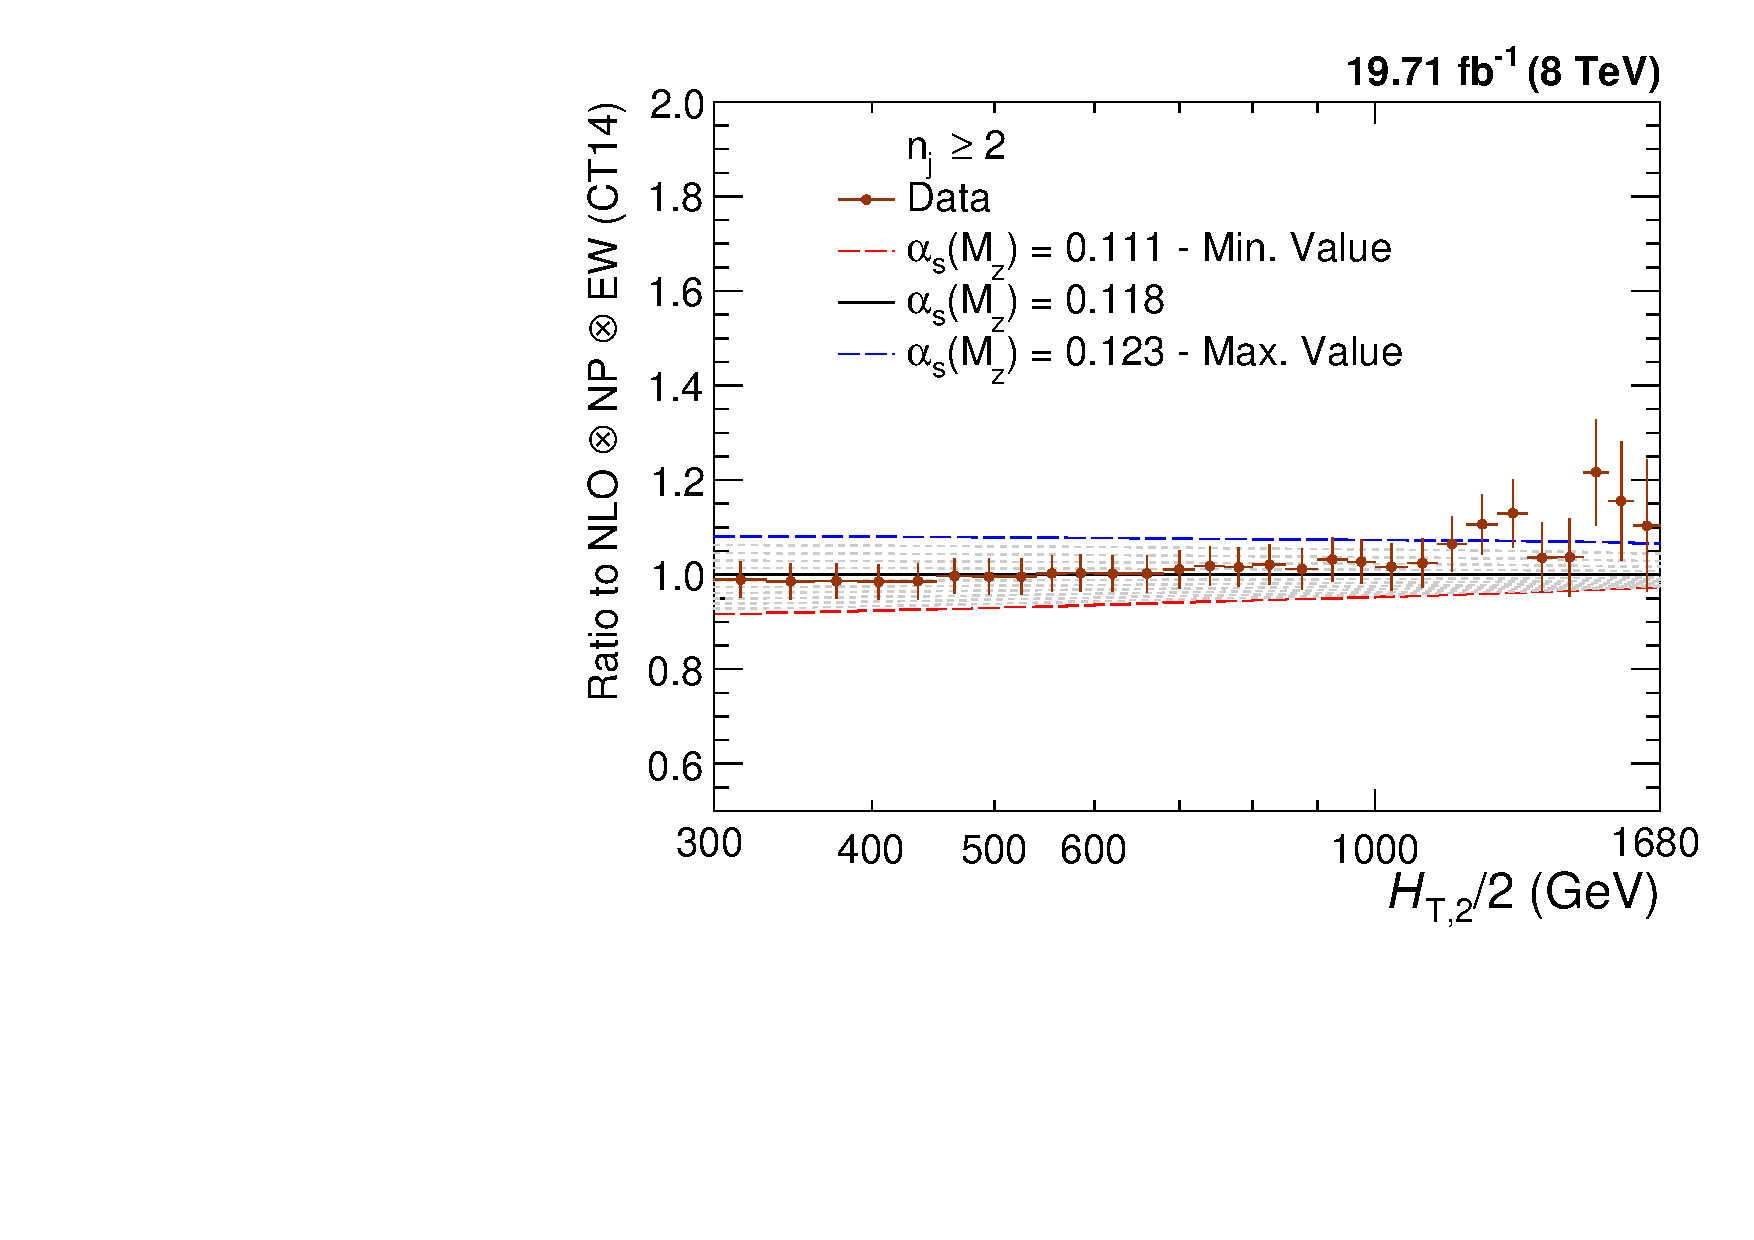
\includegraphics[width=0.51\textwidth]{Plots_HT_2_150/Sensitivity_2_ratio_NLO_CT14_EW.pdf}\\
 \vspace*{3mm}
 \hspace*{-5mm}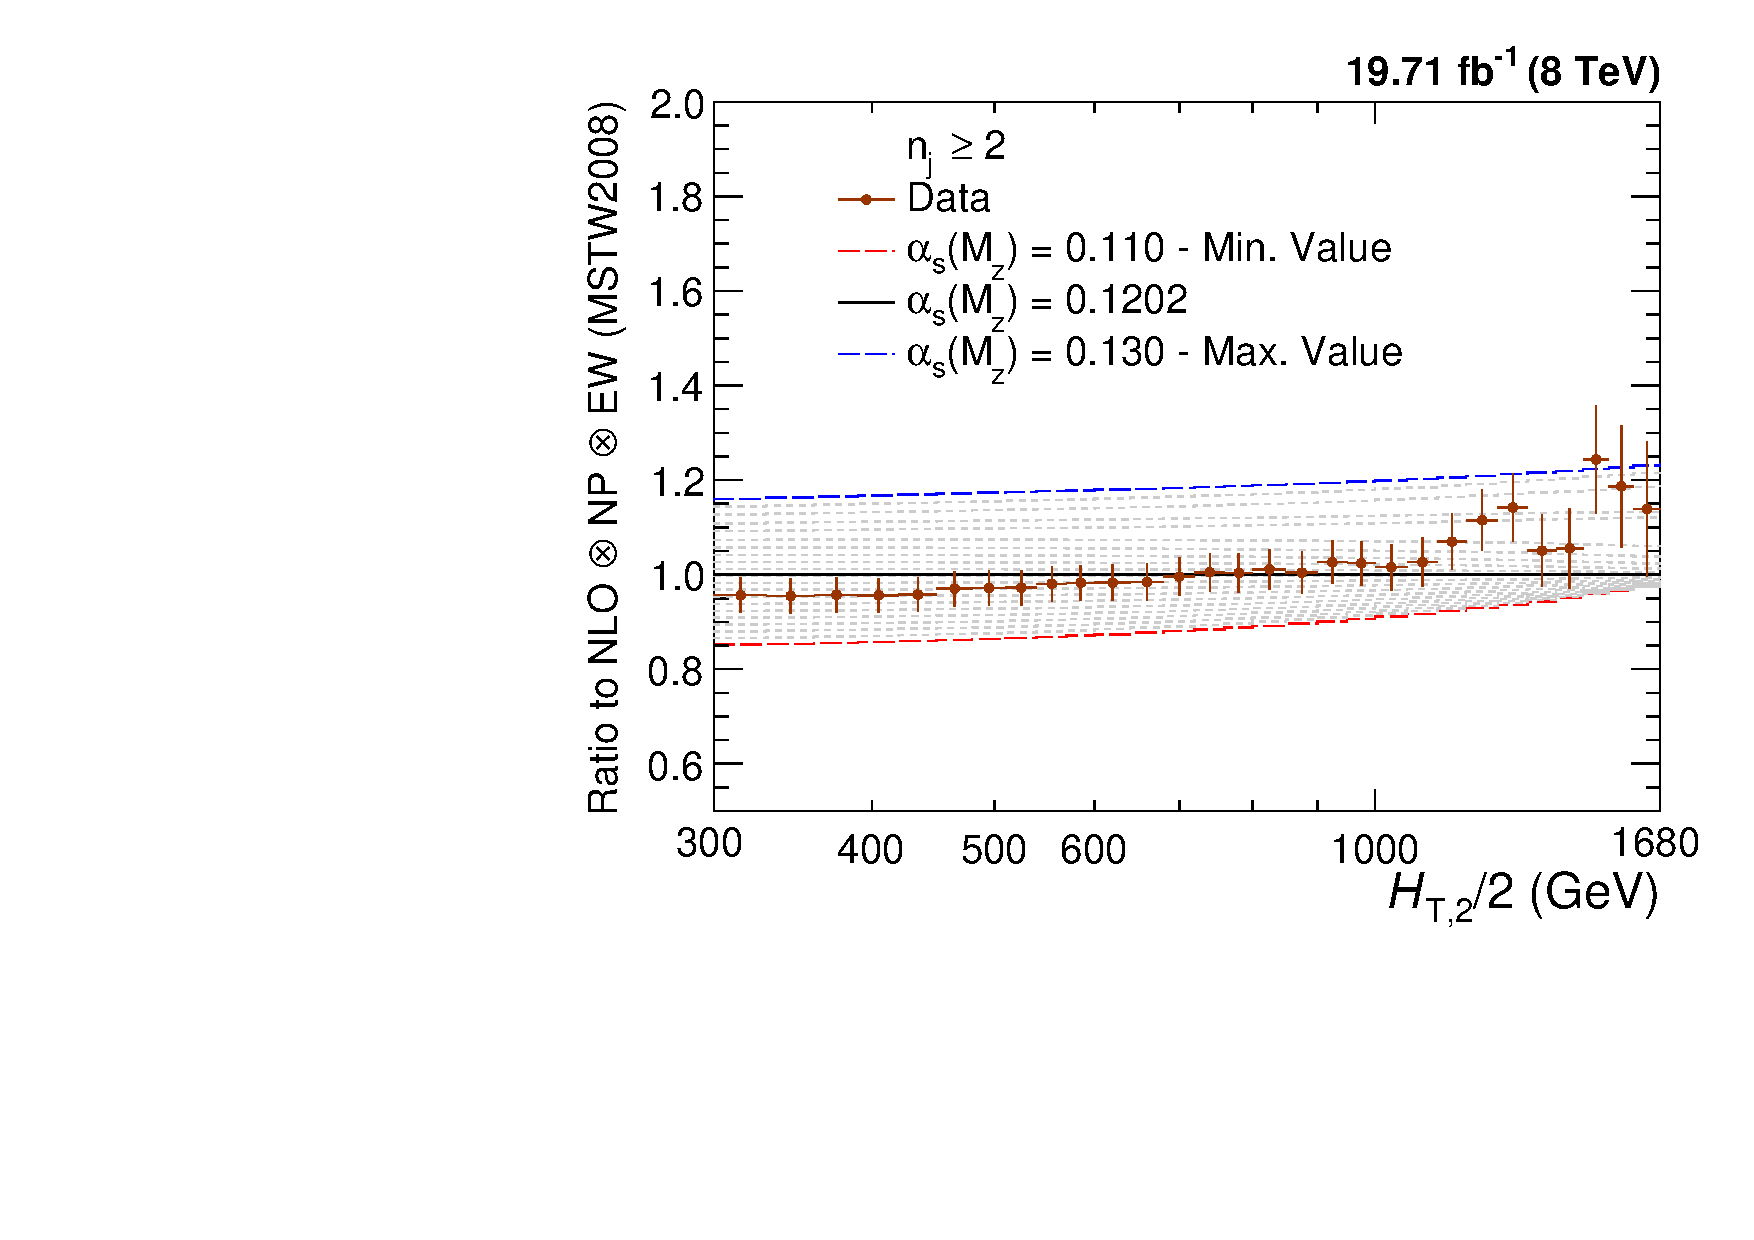
\includegraphics[width=0.51\textwidth]{Plots_HT_2_150/Sensitivity_2_ratio_NLO_MSTW2008_EW.pdf}%
 ~~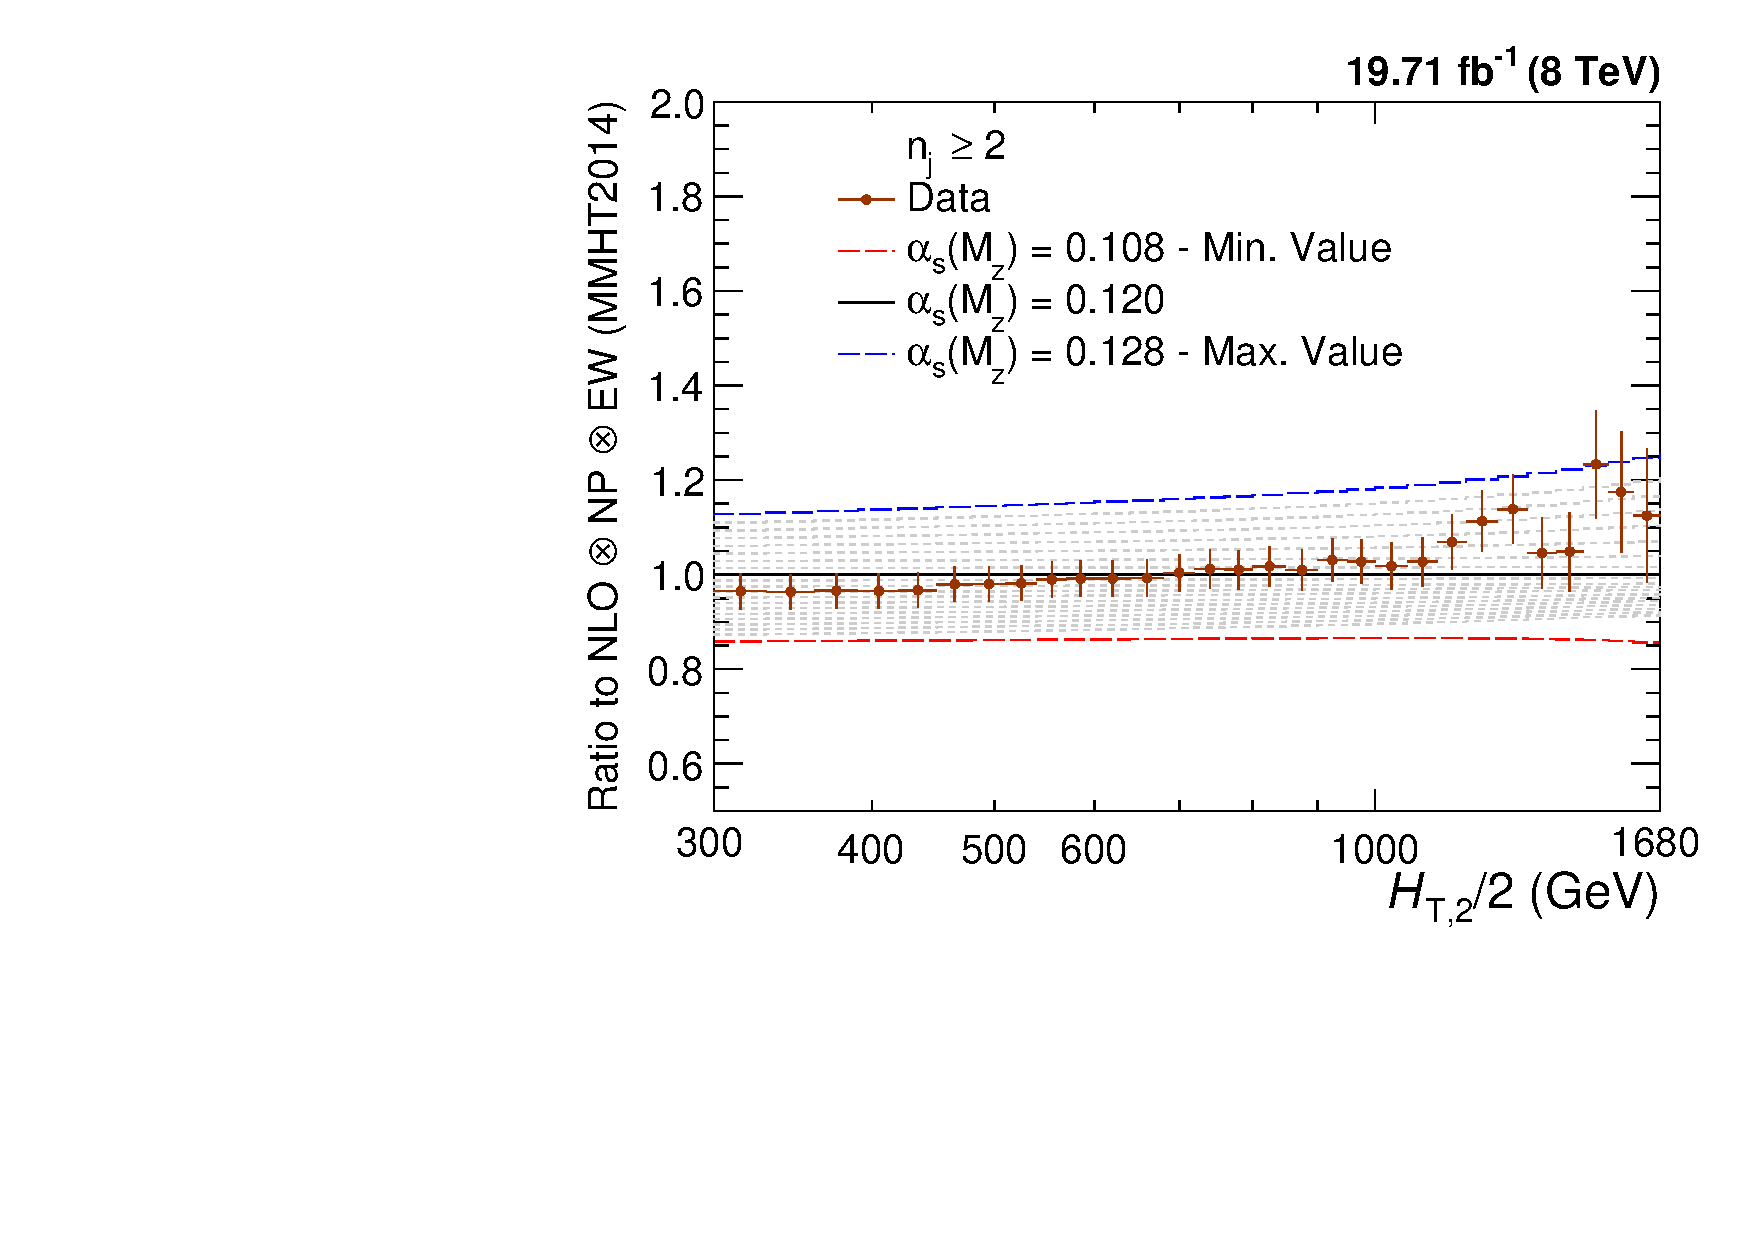
\includegraphics[width=0.51\textwidth]{Plots_HT_2_150/Sensitivity_2_ratio_NLO_MMHT2014_EW.pdf}\\
 \vspace*{3mm}
 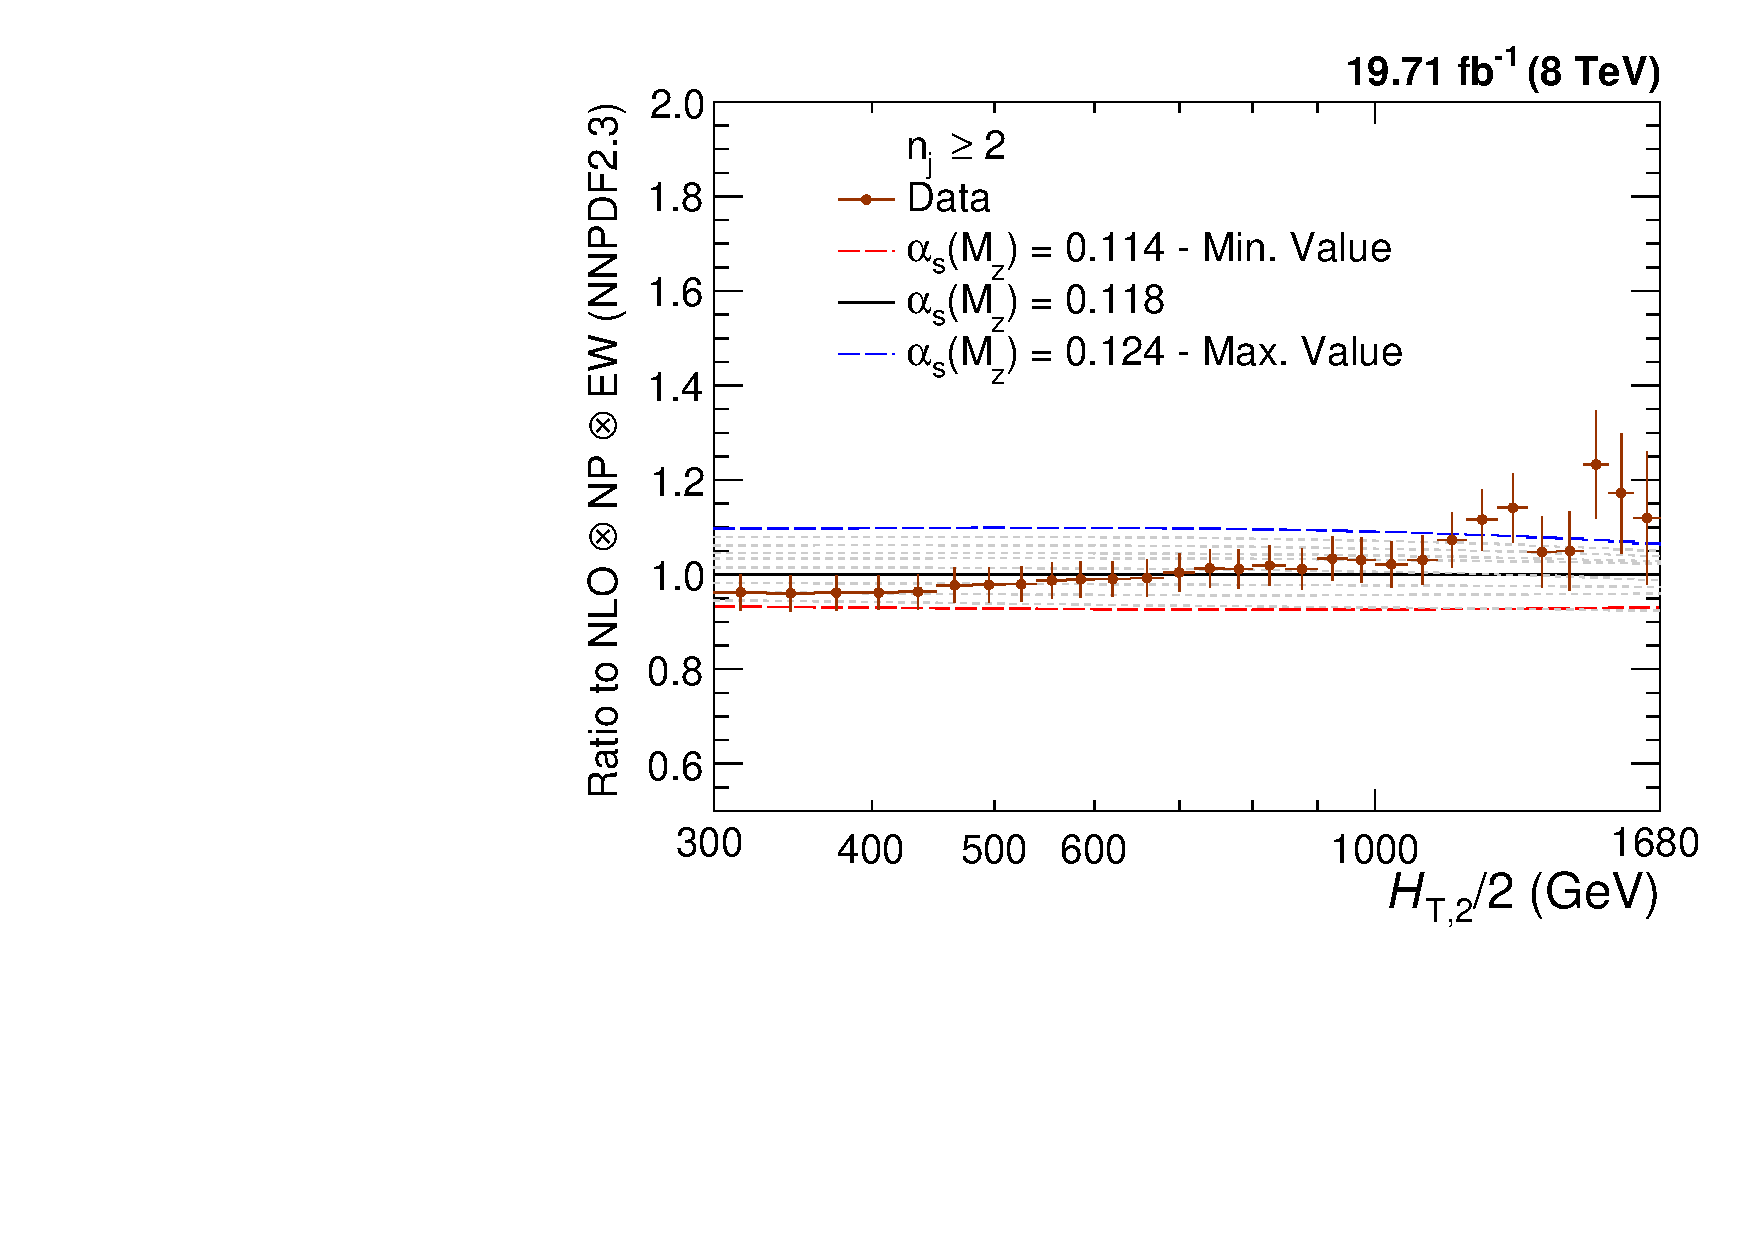
\includegraphics[width=0.51\textwidth]{Plots_HT_2_150/Sensitivity_2_ratio_NLO_NNPDF23_EW.pdf}
 \caption{Ratio of the inclusive 2-jet differential cross-section to theory predictions using the CT10 (top left), the CT14 (top right), the MSTW2008 (middle left), the MMHT2014 (middle right) and NNPDF2.3 (bottom) NLO PDF sets for a series of values of \alpsmz. The \alpsmz value is varied in the range 0.112-0.127, 0.111-123, 0.110-0.130, 0.108-0.128 and 0.114-0.124 in steps of 0.001 for the CT10, CT14, MSTW2008, MMHT2014 and NNPDF2.3 NLO PDF sets, respectively. The error bars correspond to the total experimental uncertainty. The theory predictions are corrected for non-perturbative (NP) and electroweak (EW) effects.}
 \label{fig:sensitivity_2}
 \end{center}
\end{figure}

\begin{figure}[!htbp]
 \begin{center}
 \hspace*{-5mm}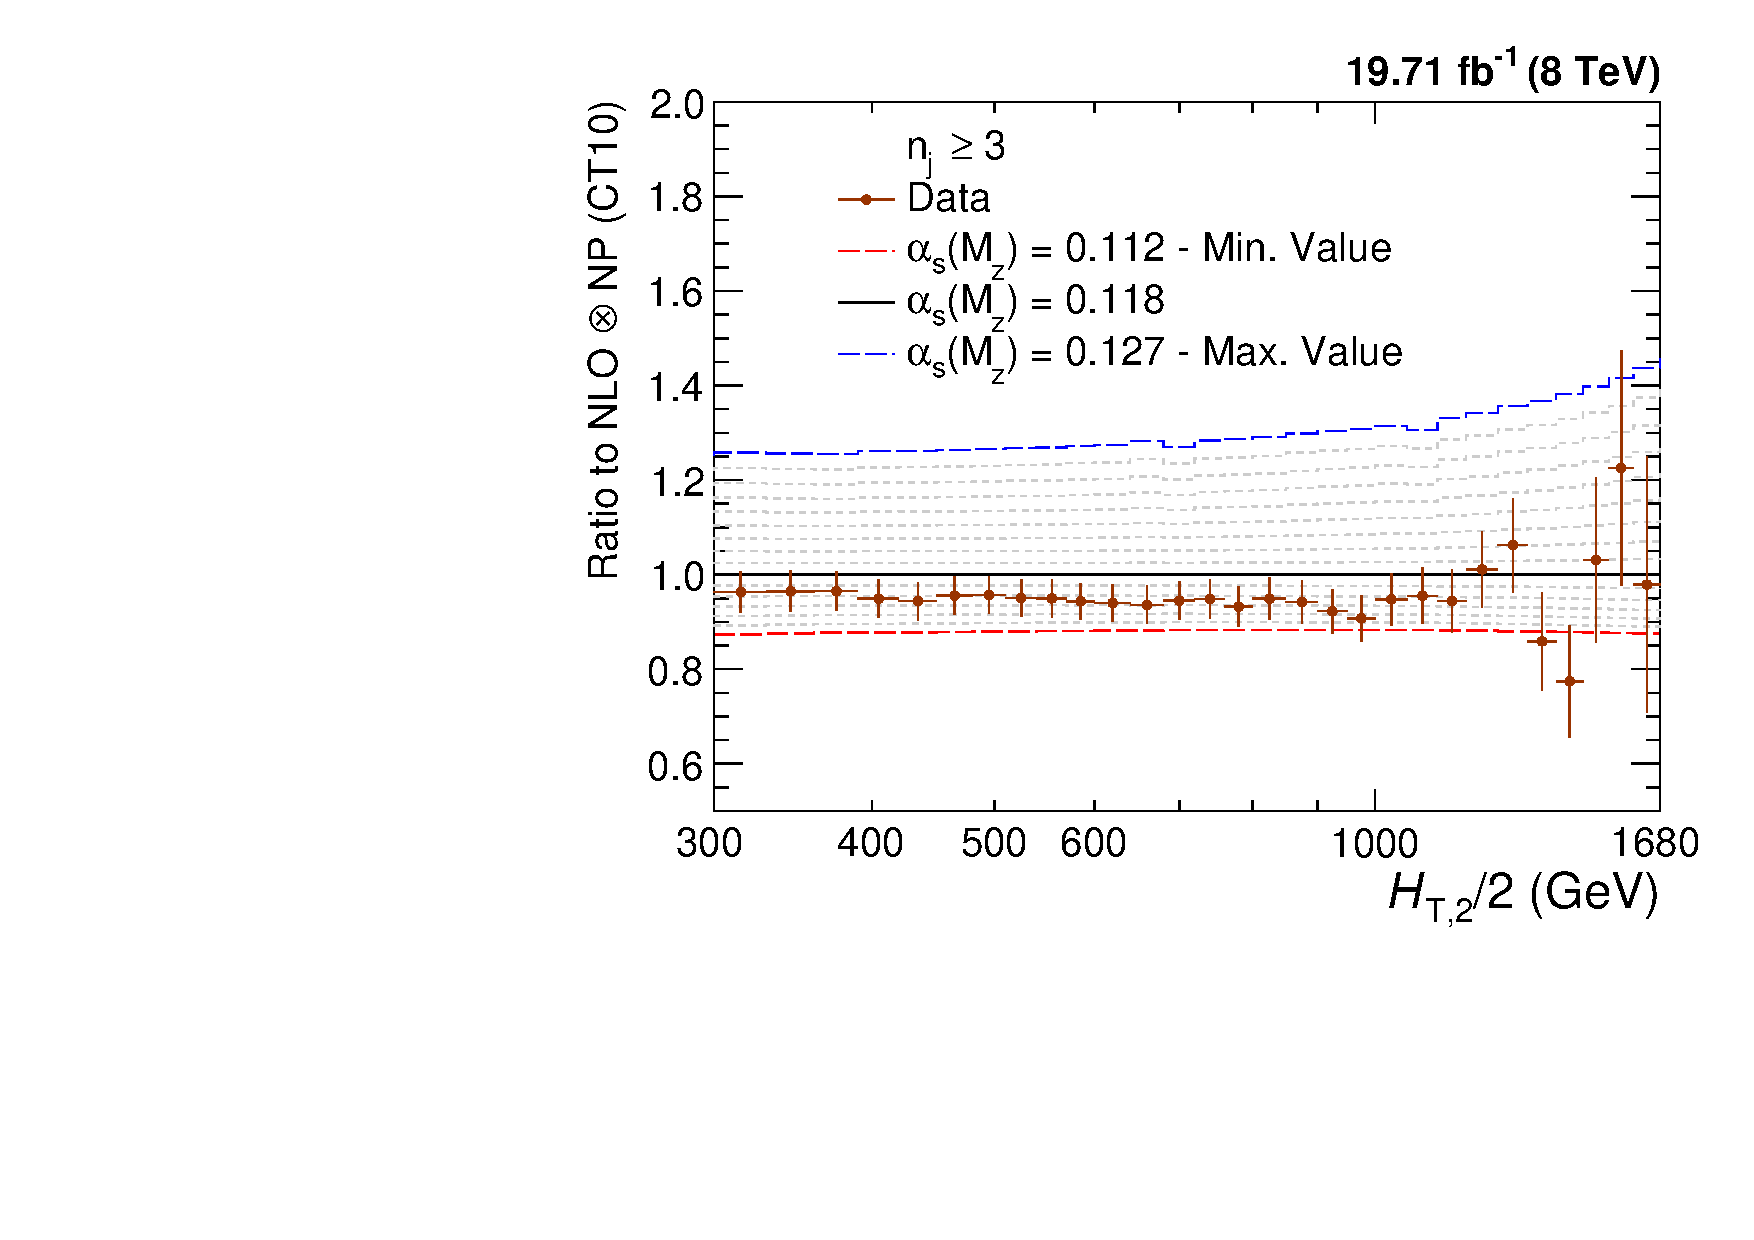
\includegraphics[width=0.51\textwidth]{Plots_HT_2_150/Sensitivity_3_ratio_NLO_CT10.pdf}%
 ~~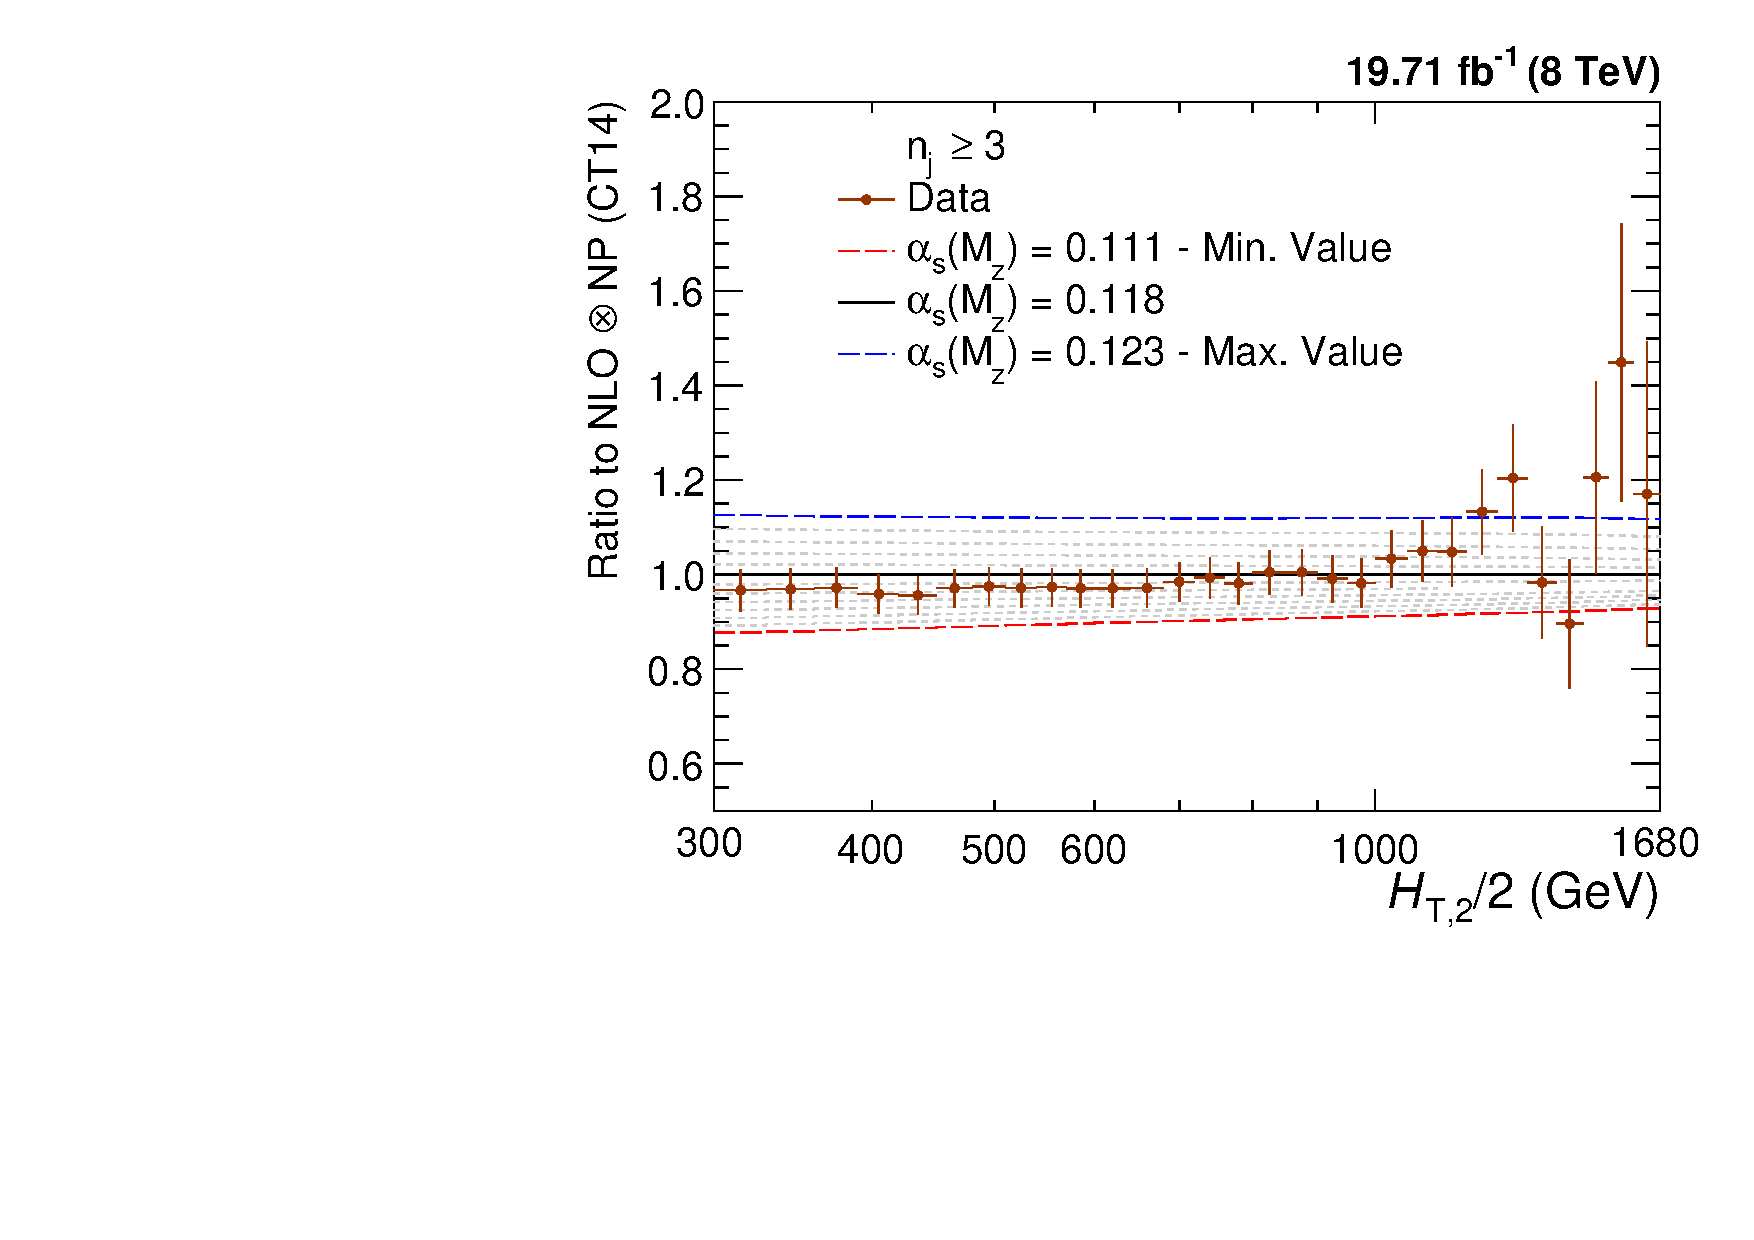
\includegraphics[width=0.51\textwidth]{Plots_HT_2_150/Sensitivity_3_ratio_NLO_CT14.pdf}\\
 \vspace*{3mm}
 \hspace*{-5mm}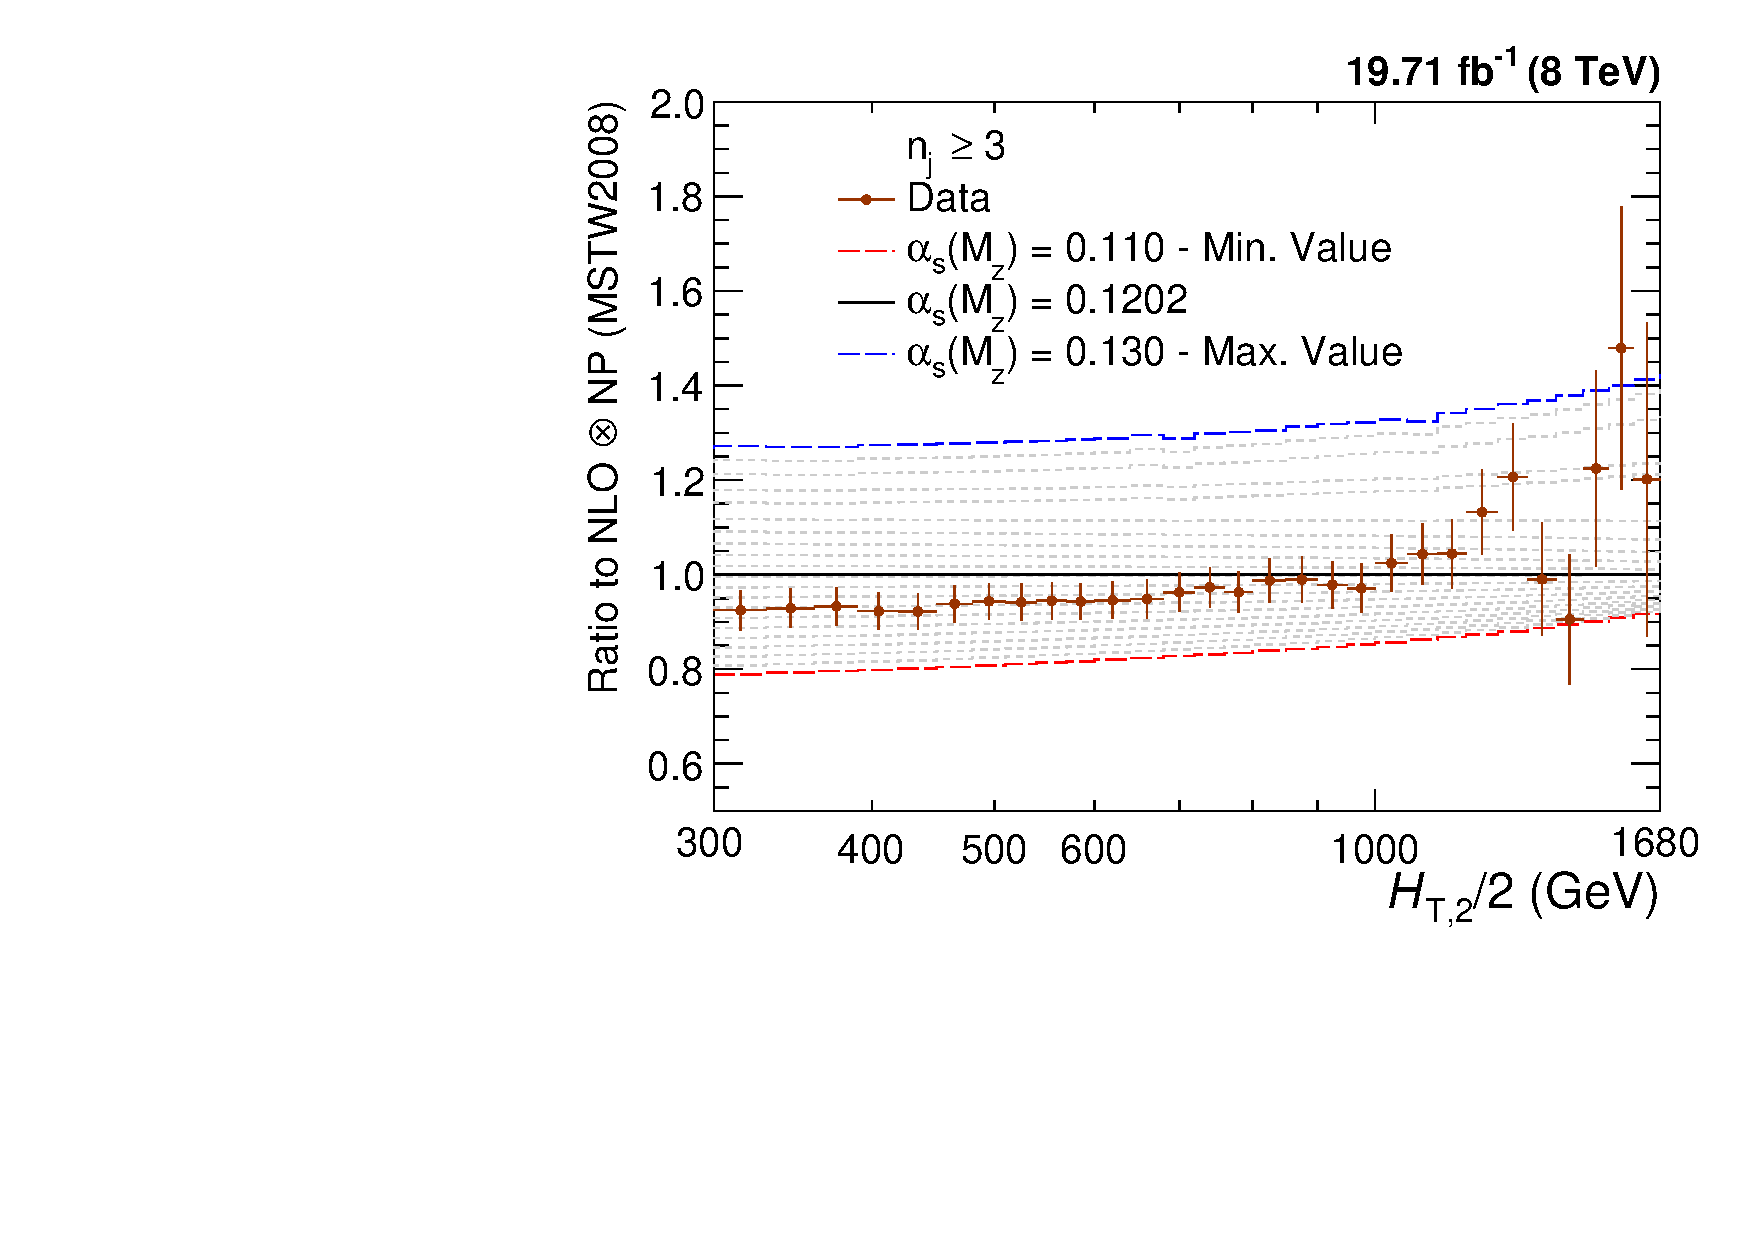
\includegraphics[width=0.51\textwidth]{Plots_HT_2_150/Sensitivity_3_ratio_NLO_MSTW2008.pdf}%
 ~~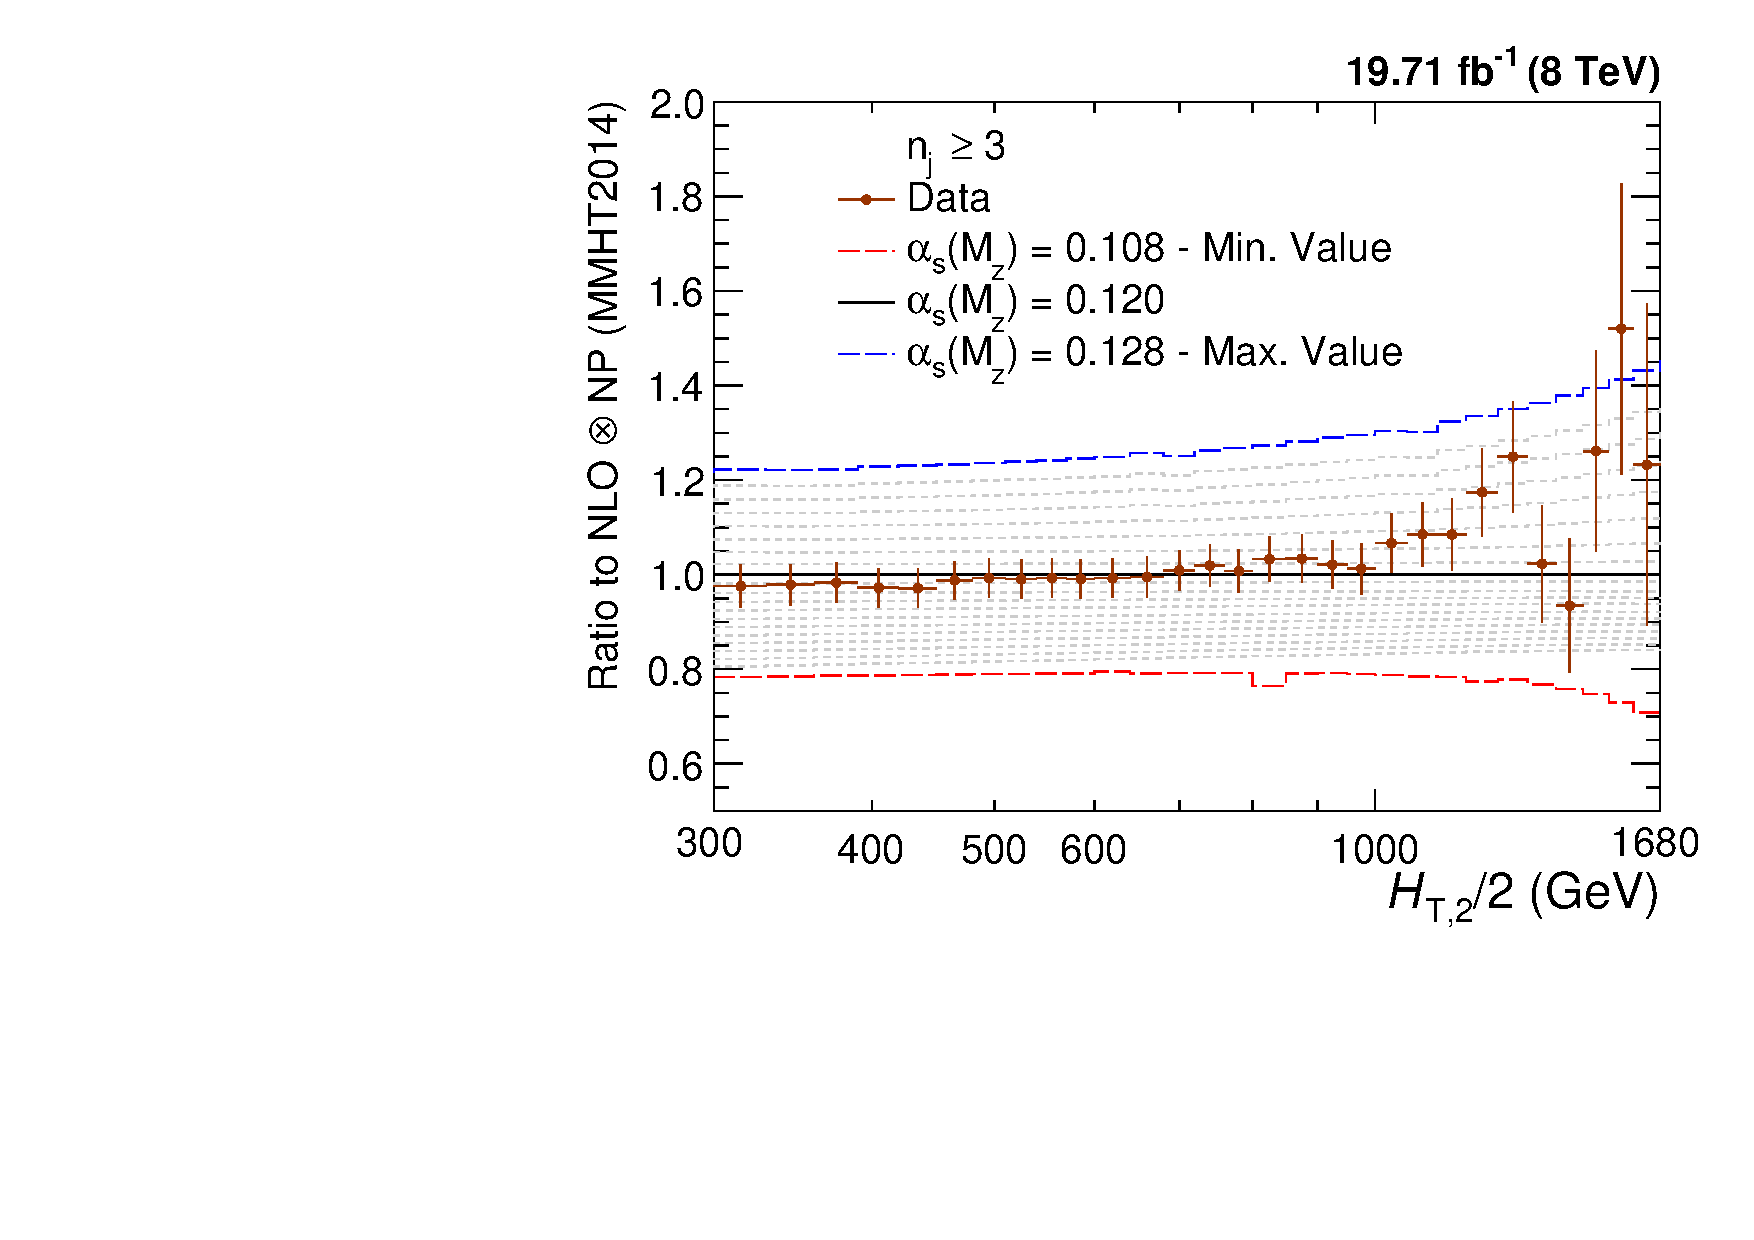
\includegraphics[width=0.51\textwidth]{Plots_HT_2_150/Sensitivity_3_ratio_NLO_MMHT2014.pdf}\\
 \vspace*{3mm}
 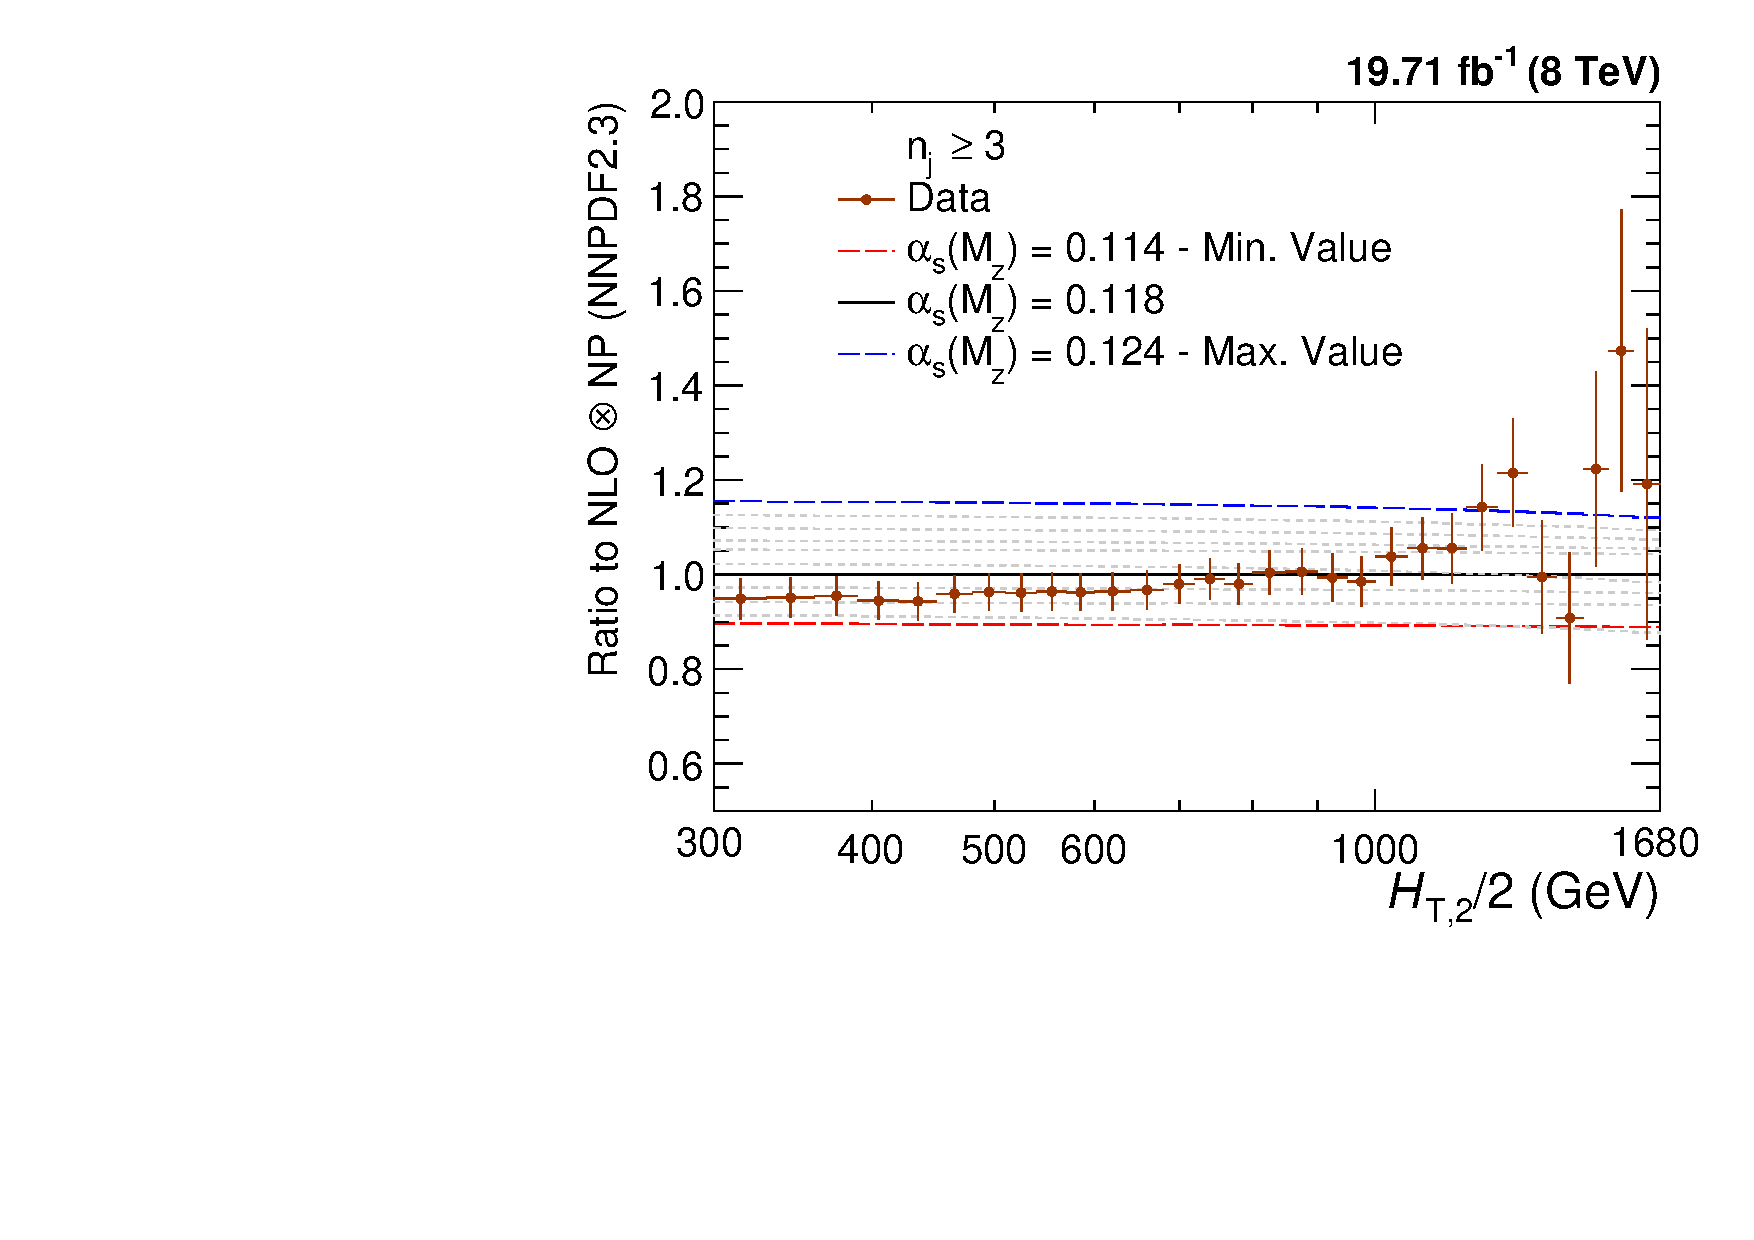
\includegraphics[width=0.51\textwidth]{Plots_HT_2_150/Sensitivity_3_ratio_NLO_NNPDF23.pdf}
 \caption{Ratio of the inclusive 3-jet differential cross-section to theory predictions using the CT10 (top left), the CT14 (top right), the MSTW2008 (middle left), the MMHT2014 (middle right) and NNPDF2.3 (bottom) NLO PDF sets for a series of values of \alpsmz. The \alpsmz value is varied in the range 0.112-0.127, 0.111-123, 0.110-0.130, 0.108-0.128 and 0.114-0.124 in steps of 0.001 for the CT10, CT14, MSTW2008, MMHT2014 and NNPDF2.3 NLO PDF sets, respectively. The error bars correspond to the total experimental uncertainty. The theory predictions are corrected for non-perturbative (NP) effects.}
 \label{fig:sensitivity_3}
 \end{center}
\end{figure}

\begin{figure}[!htbp]
 \begin{center}
 \hspace*{-5mm}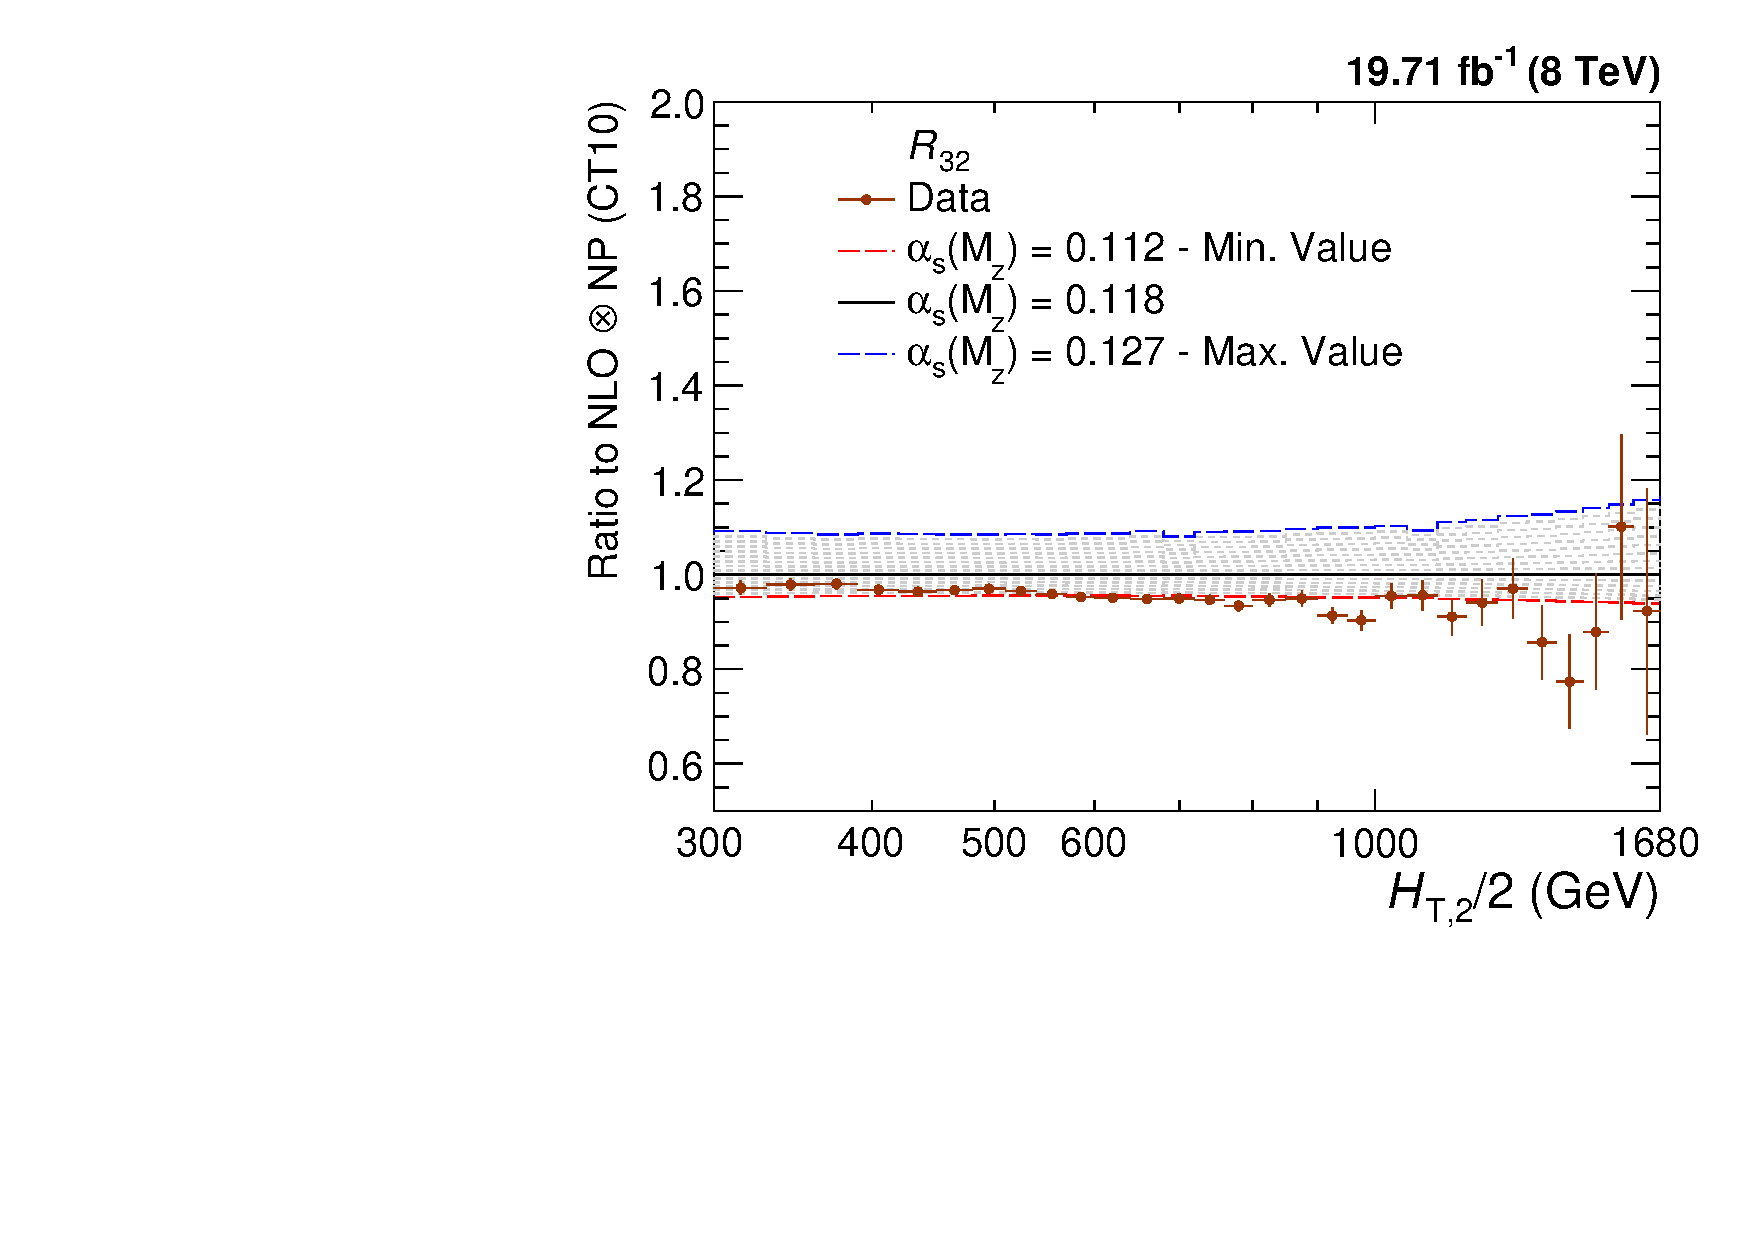
\includegraphics[width=0.51\textwidth]{Plots_HT_2_150/Sensitivity_double_ratio_32_CT10.pdf}%
 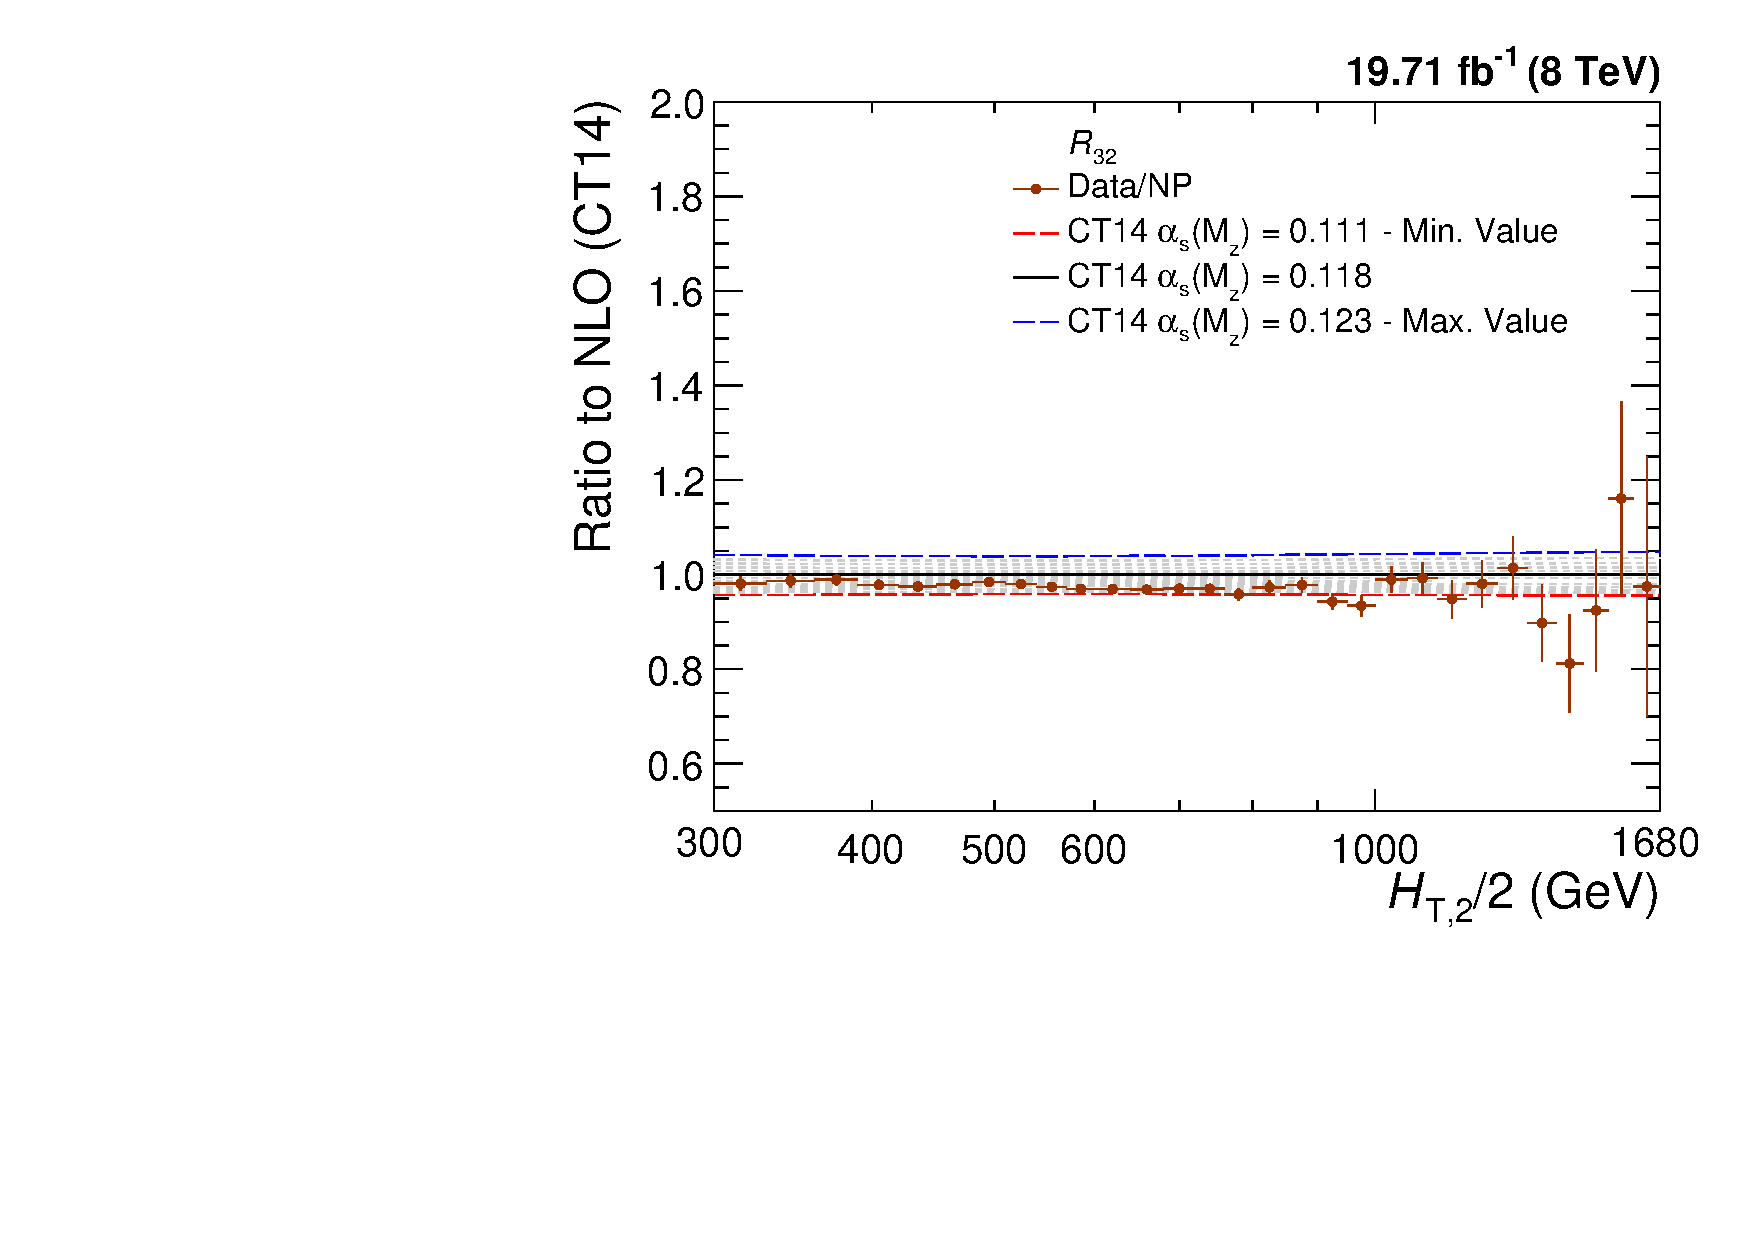
\includegraphics[width=0.51\textwidth]{Plots_HT_2_150/Sensitivity_double_ratio_32_CT14.pdf}\\
 \vspace*{3mm}
 \hspace*{-5mm}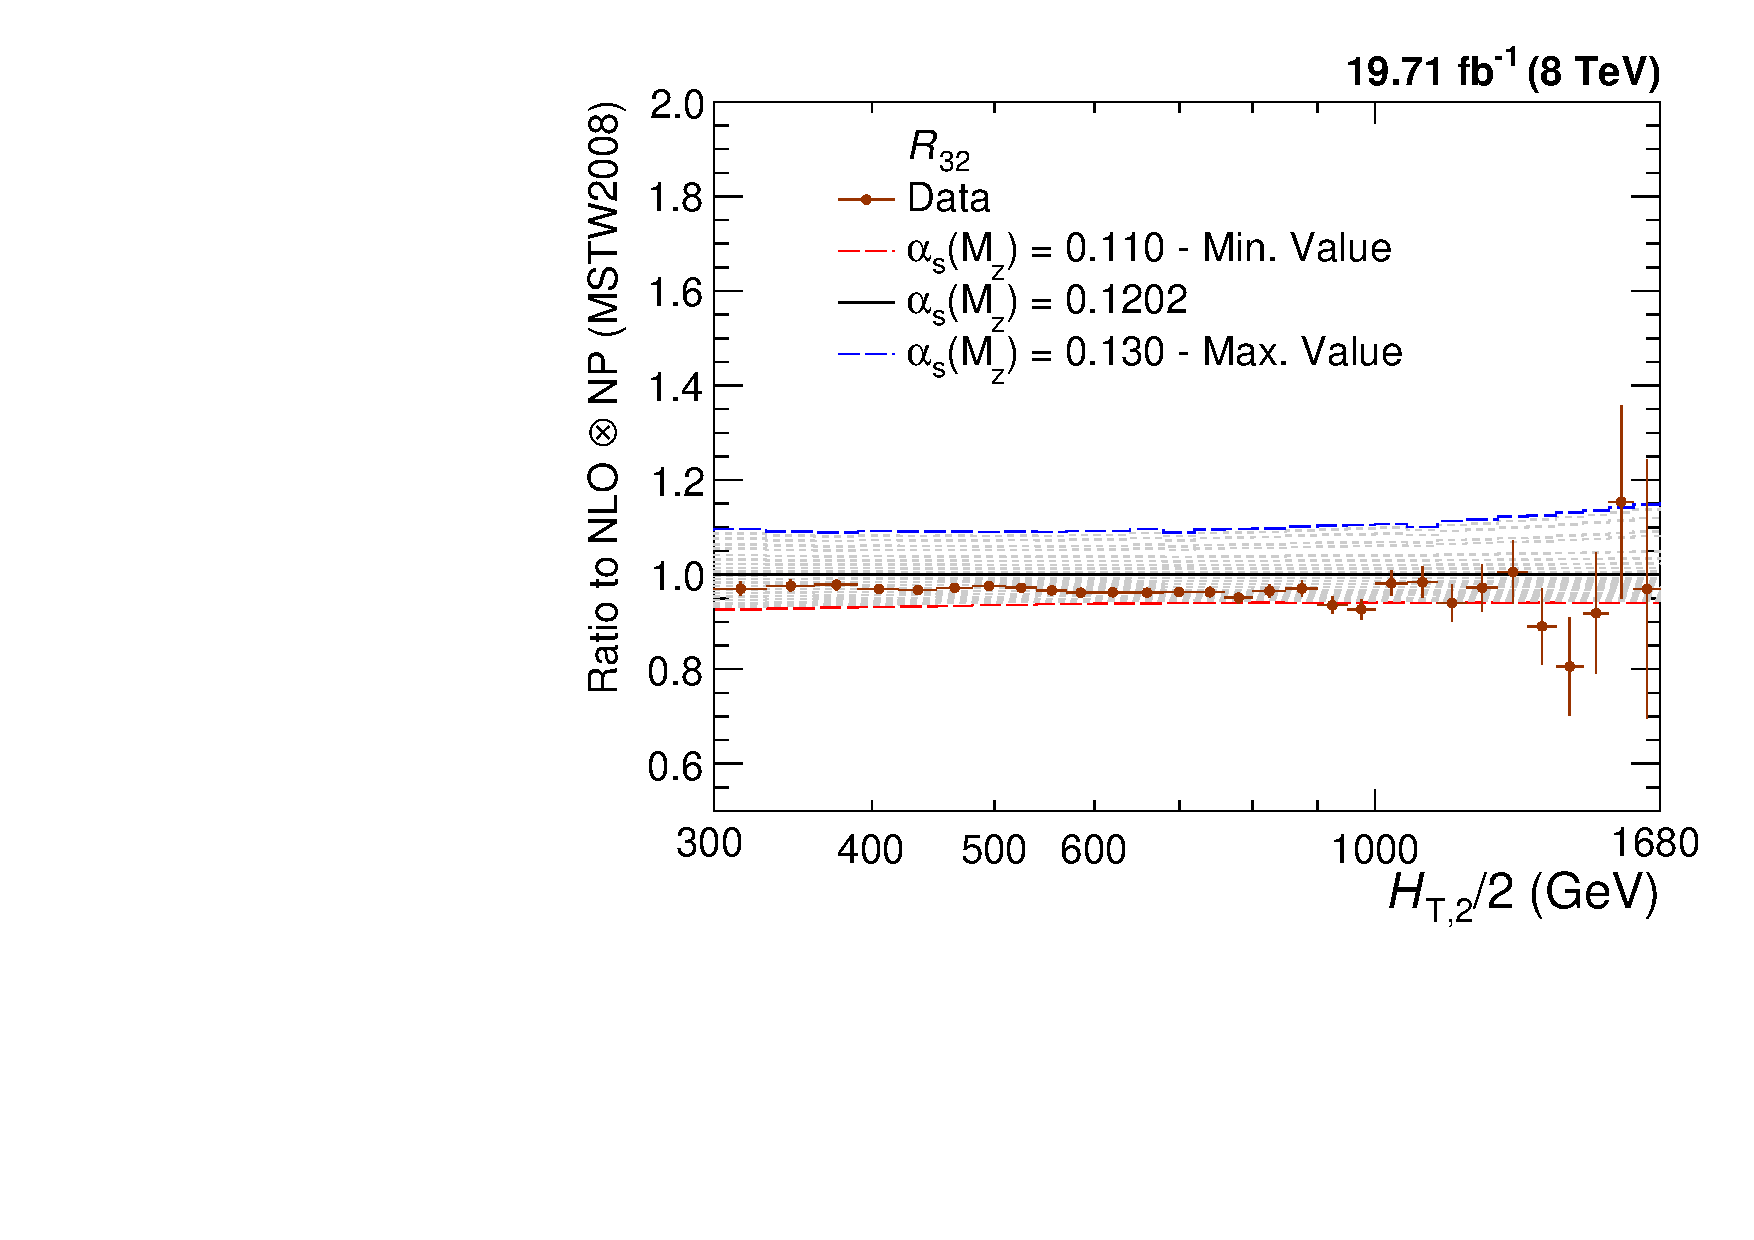
\includegraphics[width=0.51\textwidth]{Plots_HT_2_150/Sensitivity_double_ratio_32_MSTW2008.pdf}%
 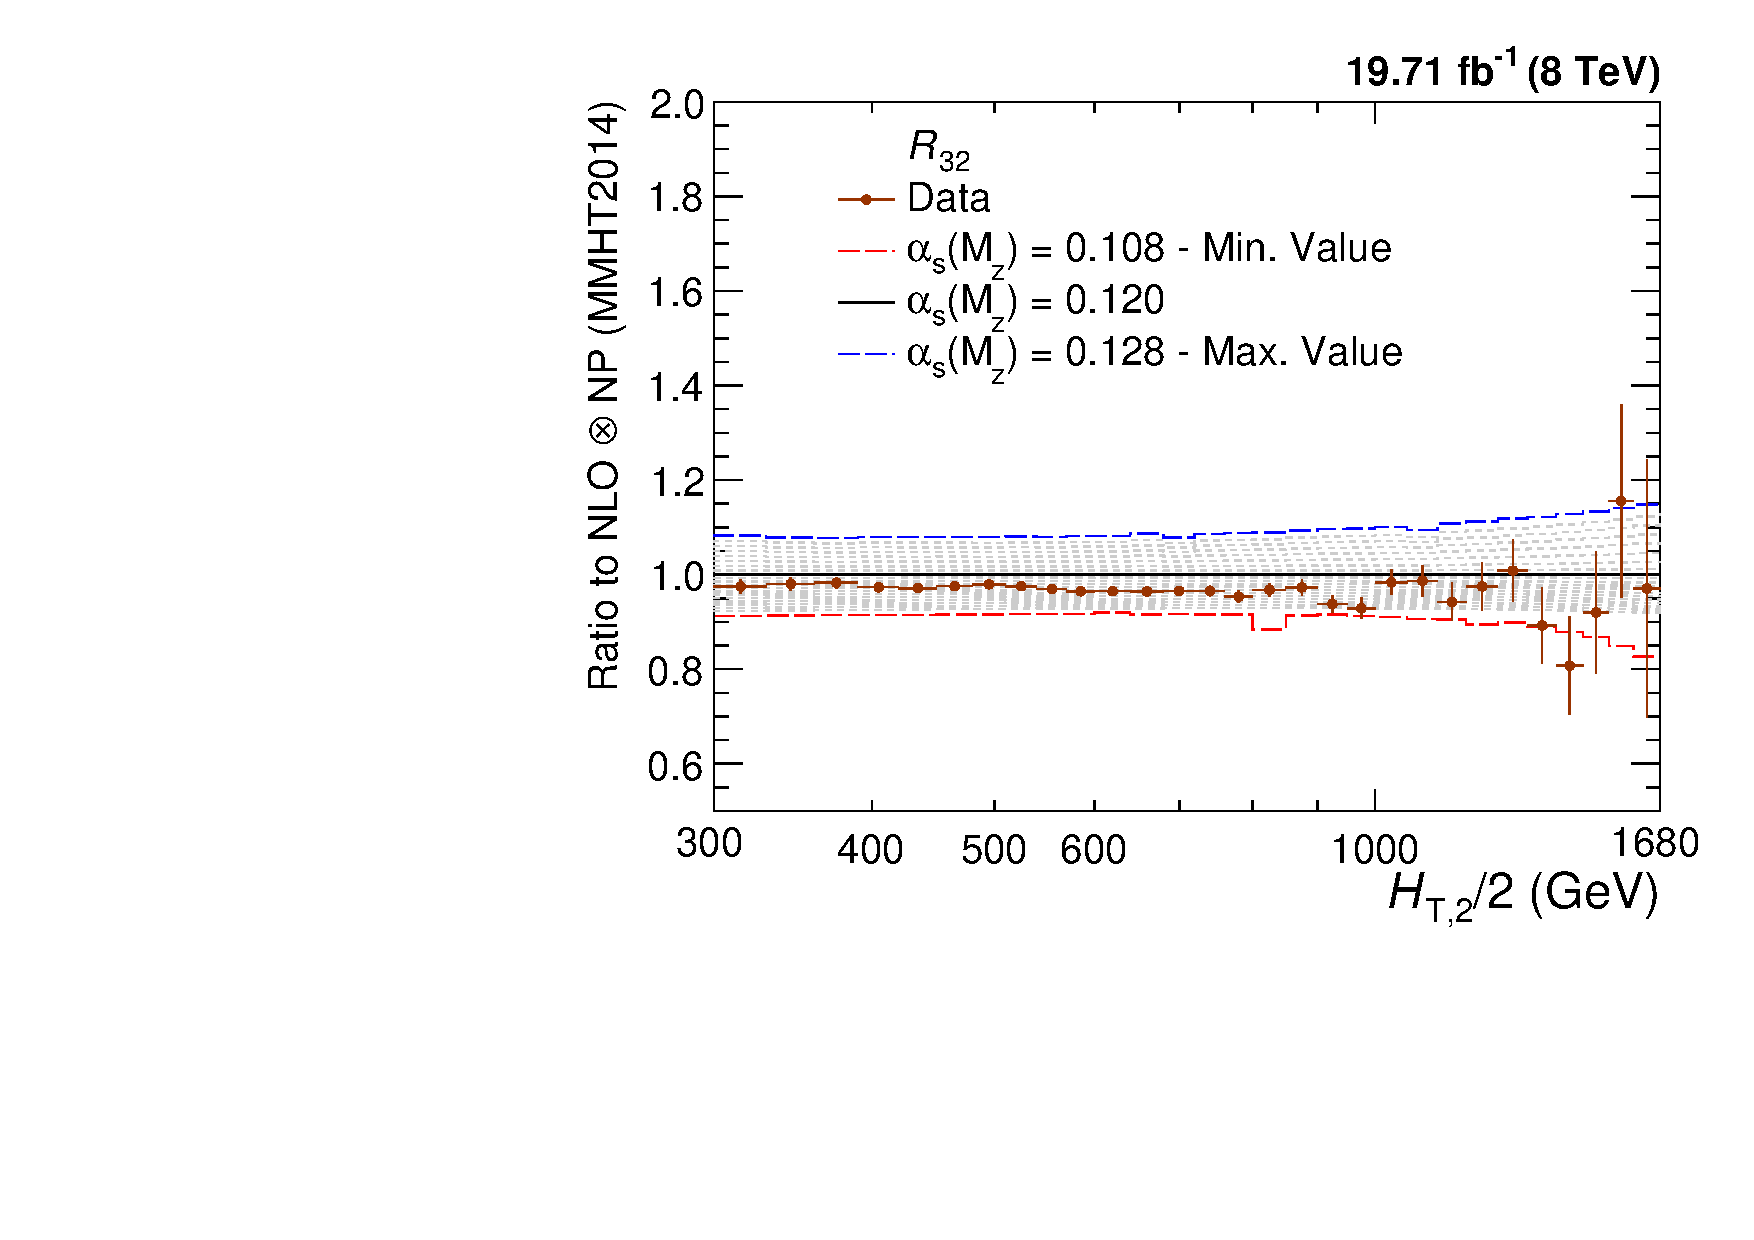
\includegraphics[width=0.51\textwidth]{Plots_HT_2_150/Sensitivity_double_ratio_32_MMHT2014.pdf}\\
 \vspace*{3mm}
 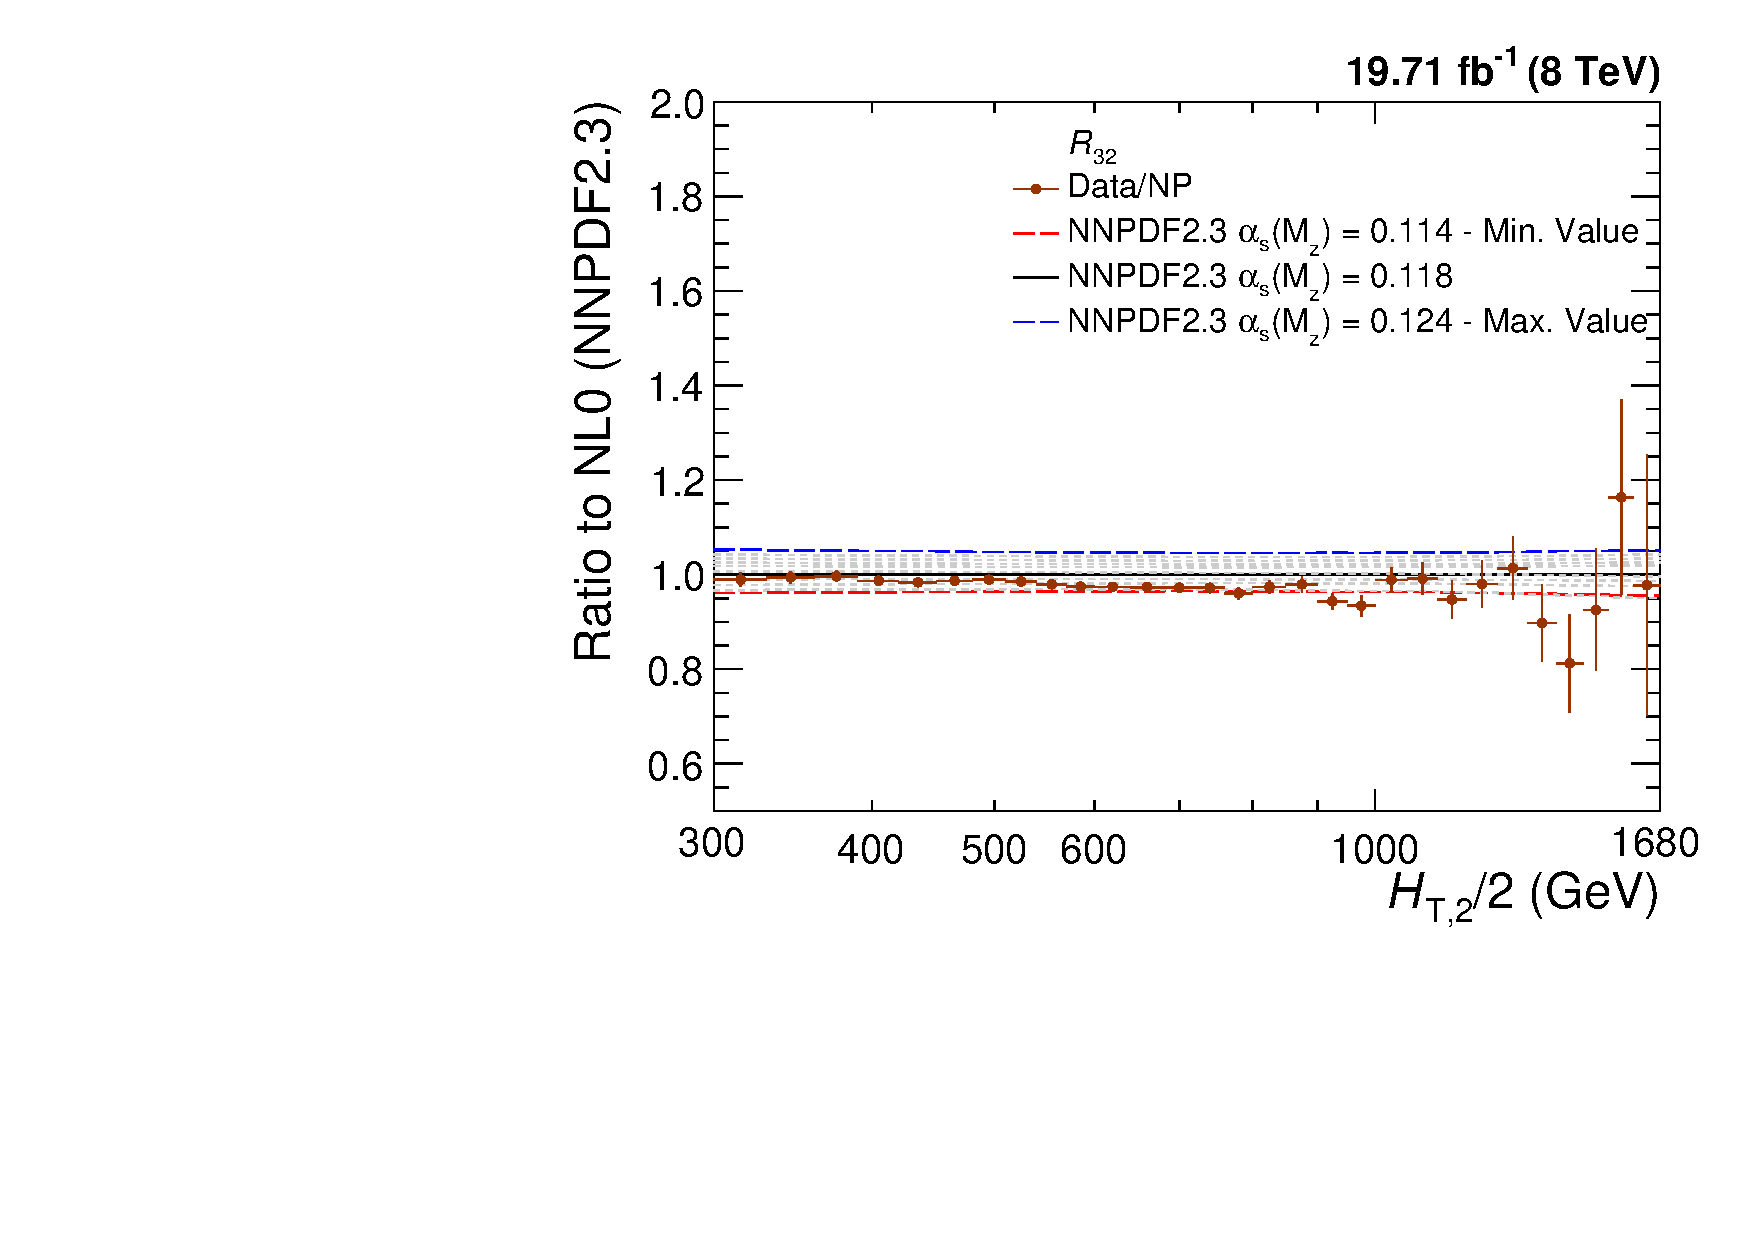
\includegraphics[width=0.51\textwidth]{Plots_HT_2_150/Sensitivity_double_ratio_32_NNPDF23.pdf}
 \caption{Ratio of the cross-section ratio, \ratio to theory predictions using the CT10 (top left), the CT14 (top right), the MSTW2008 (middle left), the MMHT2014 (middle right) and NNPDF2.3 (bottom) NLO PDF sets for a series of values of \alpsmz. The \alpsmz value is varied in the range 0.112-0.127, 0.111-123, 0.110-0.130, 0.108-0.128 and 0.114-0.124 in steps of 0.001 for the CT10, CT14, MSTW2008, MMHT2014 and NNPDF2.3 NLO PDF sets, respectively. The error bars correspond to the total experimental uncertainty. The theory predictions are corrected for non-perturbative (NP) effects.}
 \label{fig:sensitivity_double_ratio}
 \end{center}
\end{figure}

\section{Determination of \texorpdfstring{\alpsmz}{alpha-S(M(Z))}}

As discussed in the previous section, the measured inclusive 2-jet and 3-jet event cross-sections and their ratio \ratio can be used for a determination of the strong coupling constant \alpsmz. To extract the value of \alpsmz, a general fit procedure \cite{Chatrchyan:2013txa,Khachatryan:2014waa} has been followed and is described in the following section. 

\subsection{Fitting Procedure}
\label{sec:Fits_procedure}
The value of \alpsmz is determined by minimizing the chi-square (\chisq) between the experimental measurement and the theoretical predictions. The \chisq is defined as:

\begin{equation}
  \label{chisq}
  \chisq = M^{T}C^{-1}M
\end{equation}
where $M$ is the vector of the differences between the data ($D^{i}$) and the theoretical values ($T^{i}$) in each bin $i$,

\begin{equation}
 \label{eqn:M_matrix}
 M^{i}=D^{i}-T^{i}
\end{equation}
and $C$ is the covariance matrix including all experimental uncertainties as described in Sec.~\ref{sec:exp_unc} and some theoretical uncertainties discussed in Sec.~\ref{sec:theory_unc}. The covariance matrix $C=C_\mathrm{exp}~\plus C_\mathrm{theo}$ is defined as the sum of covariances of experimental and theoretical sources of uncertainty as follows : 

\begin{eqnarray}
 \label{eqn:c_exp}
 C_\mathrm{exp} &=& \mathrm{Cov}^\mathrm{ExpStat}~\plus \sum\mathrm{Cov}^\mathrm{JEC}~\plus \mathrm{Cov}^\mathrm{Unfolding}~\plus \mathrm{Cov}^\mathrm{Lumi}~\plus \mathrm{Cov}^\mathrm{Residual}\\
 C_\mathrm{theo} &=& \mathrm{Cov}^\mathrm{TheoStat}~\plus \mathrm{Cov}^\mathrm{NP}~\plus \mathrm{Cov}^\mathrm{PDF}
 \label{eqn:c_theo}
\end{eqnarray}
where the labelled covariance matrices account for the following effects:

\begin{itemize}
\item{$\mathrm{Cov}^\mathrm{ExpStat}$: statistical uncertainty of the data including correlations introduced by the unfolding}
\item{$\mathrm{Cov}^\mathrm{JEC}$: the jet energy corrections (JEC) systematic uncertainty}
\item{$\mathrm{Cov}^\mathrm{Unfolding}$: the unfolding systematic uncertainty including the resolution (JER) and model dependence}
\item{$\mathrm{Cov}^\mathrm{Lumi}$: the luminosity uncertainty}
\item{$\mathrm{Cov}^\mathrm{Residual}$: a residual uncorrelated systematic uncertainty summarizing individual causes such as small trigger and identification inefficiencies, time dependence of the jet \pt resolution, and uncertainty on the trigger prescale factors}
\item{$\mathrm{Cov}^\mathrm{TheoStat}$: statistical uncertainty caused by numerical integrations in the cross-section computations}
\item{$\mathrm{Cov}^\mathrm{NP}$: the systematic uncertainty of the non-perturbative (NP) corrections}
\item{$\mathrm{Cov}^\mathrm{PDF}$: the PDF uncertainties}
\end{itemize}

While taking the differences between theory and data, the treatment of experimental and theoretical systematic uncertainties is crucial. The Unfolding, JEC, Lumi and PDF and NP systematic uncertainties are treated as 100$\%$ correlated among \httwo bins. If $\delta_i$ is the total uncertainty on the differential cross-section, for the $i$-th \httwo bin, for any of these fully correlated sources, then the$i,j$-th element of the corresponding covariance matrix is given by COV$_{ij} = \delta_i \times \delta_j$. The JEC, unfolding, and luminosity uncertainties are treated as multiplicative to avoid the statistical bias that arises when estimating uncertainties from data. In fits of the ratio \ratio, the luminosity and residual uncorrelated uncertainties cancel completely. Partial cancellations between the other sources of uncertainty are taken into account in the fit. 

The evaluation of PDF uncertainty depends on the individual PDF set as already discussed in Sec.~\ref{sec:pdf_unc}. The PDF covariance matrix construction varies among different PDF sets. The CT10, CT14, MMHT2014 and MSTW2008 NLO PDF sets employ the eigenvector method to evaluate the PDF uncertainties as explained in Sec.~\ref{sec:pdf_unc}. The number of eigenvectors ($N_\mathrm{ev}$) with two PDF members per eigenvector for CT10, CT14, MMHT2014 and MSTW2008 NLO PDF sets are 26, 28, 25 and 20, respectively. The NNPDF2.3 PDF set comes with hundred different replicas ($N_{rep}$) instead of different eigenvectors, as for CT10 or CT14 PDF sets. The mean uncertainty is calculated as average uncertainty from 100 different replicas. Following the prescription given in~\cite{Ball:2010de}, the PDF uncertainty is calculated as :

\begin{equation}
(\Delta X)^2 = \frac{1}{N_{rep}-1} \sum_{k=1}^{N_{rep}} [X_k - \langle X_k \rangle]^2
\end{equation}

where $\Delta X$ is the uncertainty on predicted differential cross-section, $X_k$ is the differential cross-section for $k$-th replica and $\langle X_k \rangle$ is the average differential cross-section from all the replicas. 

Scale uncertainties of the pQCD predictions are taken into account by employing the offset method, \ie by performing separate fits with varying scale factors as described in the Sec.~\ref{sec:scale_unc}. The largest upwards and downwards deviations from the default factors are defined as the uncertainty. At NLO such scale variations predominantly lead to smaller cross-sections and also a smaller ratio \ratio as visible in Fig.~\ref{fig:theory_unc}. As a consequence the scale uncertainty in fits is equally asymmetric, where smaller cross-sections or ratios are compensated by an increase in the fitted value for \alpsmz.

\subsection{Fit Results}
To determine the value of the strong coupling constant at the scale of the Z boson mass \alpsmz, fits to the differential inclusive 2-jet and 3-jet events cross-sections are performed using five different NLO PDF sets : CT10, CT14, MSTW2008, MMHT2014 and NNPDF2.3. The range in \httwo is restricted to be between 300 GeV and 1 TeV to avoid the region close to the minimal \pt threshold of 150 GeV for each jet at low \pt and the onset of electroweak effects at high \httwo, which are available for the dijet case only. The \alpsmz results obtained from a simultaneous fit to all 19 \httwo bins in the above mentioned range are reported in Table~\ref{tab:xsep300-1000}. For comparison, a simultaneous fit to both cross-sections ignoring any correlations, and a fit to the cross-section ratio \ratio, fully accounting for correlations is also performed and the results are tabulated in Table~\ref{tab:xcomb300-1000}. The electroweak effects are assumed to cancel in the ratio as do the luminosity and the uncorrelated uncertainty.

All cross-section fits give compatible values for \alpsmz in the range of 0.115-0.118 whereas for the ratio \ratio somewhat smaller values are obtained. But for individual cross-sections, \chisqndof values are small as compared to the cross-section ratio \ratio. A possible explanation is an overestimation of the residual uncorrelated uncertainty of 1\% that is cancelled for \ratio. If the fits are repeated with an assumed uncertainty of 0.25\% instead, the \chisqndof values lie around unity while the \alpsmz values are still compatible with the previous results but with slightly reduced uncertainties. 
%
% 300 - 1000 GeV
%
\begin{table}[htbp]
 \caption{Determination of \alpsmz from the inclusive 2-jet and 3-jet event cross-sections using five PDF sets at NLO\@. Only total uncertainties without scale variations are quoted. The results are obtained from a simultaneous fit to all 19 \httwo bins in the restricted range of $0.3 < \httwo < 1.0$ TeV.}
 \label{tab:xsep300-1000}
 \centering
 \vspace{2mm} 
 \begin{tabular}{l|ccc|ccc}
 \hline\hline
 \multirow{2}{*}{PDF set} & \multicolumn{3}{c|}{Inclusive 2-jets} & \multicolumn{3}{c}{Inclusive 3-jets} \\
      & \alpsmz & $\pm\Delta\alpsmz$ & \chisqndof &\alpsmz & $\pm\Delta\alpsmz$ & \chisqndof \\\hline
 CT10           & 0.1174 & 0.0032 & 3.0/18 & 0.1169 & 0.0027 & 5.4/18 \rbtrr\\
 CT14           & 0.1160 & 0.0035 & 3.5/18 & 0.1159 & 0.0031 & 6.1/18 \rbtrr\\
 MSTW2008       & 0.1159 & 0.0025 & 5.3/18 & 0.1161 & 0.0021 & 6.7/18 \rbtrr\\
 MMHT2014       & 0.1165 & 0.0034 & 5.9/18 & 0.1166 & 0.0025 & 7.1/18 \rbtrr\\
 NNPDF2.3       & 0.1183 & 0.0025 & 9.7/18 & 0.1179 & 0.0021 & 9.1/18 \rbtrr\\
 \hline\hline
 \end{tabular}
\end{table}

\begin{table}[htbp]
 \caption{Determination of \alpsmz from the inclusive 2-jet and 3-jet event cross-sections simultaneously and from their ratio \ratio using five PDF sets at NLO\@. Only total uncertainties without scale variations are quoted. The results are obtained from a simultaneous fit to all 38 (left) and 19 (right) \httwo bins in the restricted range of $0.3 < \httwo < 1.0$ TeV. For comparison, correlations between the two cross-sections are neglected in the simultaneous fit on the left, but fully taken into account in the ratio fit on the right.}
 \label{tab:xcomb300-1000}
 \centering
 \vspace{2mm}  
 \begin{tabular}{l|ccc|ccc}
 \hline\hline
 \multirow{2}{*}{PDF set} & \multicolumn{3}{c|}{Inclusive 2- and 3-jets} & \multicolumn{3}{c}{\ratio} \\
    & \alpsmz & $\pm\Delta\alpsmz$ & \chisqndof &\alpsmz & $\pm\Delta\alpsmz$ & \chisqndof \\\hline
    CT10           & 0.1170 & 0.0026 & 8.2/37 & 0.1141 & 0.0028 & 19./18 \rbtrr\\
    CT14           & 0.1161 & 0.0029 & 9.1/37 & 0.1139 & 0.0032 & 15./18 \rbtrr\\
    MSTW2008       & 0.1161 & 0.0021 & 11./37 & 0.1150 & 0.0023 & 21./18 \rbtrr\\
    MMHT2014       & 0.1168 & 0.0025 & 11./37 & 0.1142 & 0.0022 & 19./18 \rbtrr\\
    NNPDF2.3       & 0.1188 & 0.0019 & 15./37 & 0.1184 & 0.0021 & 12./18 \rbtrr\\
    \hline\hline
  \end{tabular}
\end{table}

To investigate how the electroweak (EW) corrections affect the fit results for \alpsmz, the range in \httwo is extended to $0.3 < \httwo < 1.68$ TeV. \alpsmz values are obtained from fits to the inclusive 2-jet event cross-section in this range with or without EW correction factors and the results are presented in Table~\ref{tab:xsep300-1680}. The largest impact is a reduction in \chisqndof, which indicates a better agreement when EW effects are included. In addition, a tendency to slightly smaller \alpsmz values is observed without the EW corrections. For the ratio \ratio, it is expected that these effects are much reduced. 
%
% 300 - 1680 GeV, 2j only, w/o ew
%
\begin{table}[htbp]
 \caption{Determination of \alpsmz from the inclusive 2-jet event cross-section using five PDF sets at NLO without (left) and with (right) electroweak (EW) corrections. Only total uncertainties without scale variations are quoted. The results are obtained from a simultaneous fit to all 29 \httwo bins in the range of $0.3 < \httwo < 1.68$ TeV.}
 \label{tab:xsep300-1680}
 \centering
 \vspace{2mm}
 \begin{tabular}{l|ccc|ccc}
 \hline\hline
 \multirow{2}{*}{PDF set} & \multicolumn{3}{c|}{without EW} &
 \multicolumn{3}{c}{with EW} \\
 & \alpsmz & $\pm\Delta\alpsmz$ & \chisqndof &\alpsmz & $\pm\Delta\alpsmz$ & \chisqndof \\\hline
 CT10           & 0.1163 & 0.0034 & 15./28 & 0.1165 & 0.0032 & 14./28 \rbtrr\\
 CT14           & 0.1137 & 0.0033 & 24./28 & 0.1144 & 0.0033 & 17./28 \rbtrr\\
 MSTW2008       & 0.1093 & 0.0028 & 27./28 & 0.1133 & 0.0023 & 19./28 \rbtrr\\
 MMHT2014       & 0.1127 & 0.0032 & 32./28 & 0.1141 & 0.0032 & 21./28 \rbtrr\\
 NNPDF2.3       & 0.1162 & 0.0024 & 31./28 & 0.1168 & 0.0024 & 23./28 \rbtrr\\
 \hline\hline
 \end{tabular}
\end{table}

From Fig.~\ref{fig:sensitivity_double_ratio} follows that only the PDF sets MSTW2008 and MMHT2014 provide a large enough range in \alpsmz values to ensure fits without extrapolation. The other three PDF sets are at the limit such that reliable fits cannot be performed for all scale settings and/or bins in scale $Q=\httwo$. Since many systematic uncertainties cancel completely or partially in the cross-section ratio \ratio as compared to the individual cross-sections, \ratio is used mainly to determine the value of \alpsmz. Table~\ref{tab:xcomb300-1680} give the complete results for MSTW2008 and MMHT2014 for the full range in \httwo of 300 GeV up to 1.68 TeV along with the corresponding components of PDF, scale, NP and total experimental except scale uncertainties are shown. In contrast to fits at NLO using cross-sections where the scale uncertainty recipe usually leads to a very asymmetric behaviour with larger downward uncertainties in the case, this is inverted for the fits to the cross-section ratio \ratio. The scale uncertainty is the most dominant source of total uncertainty on \alpsmz. These values are determined with the central renormalization and factorization scales i.e. \mur = \muf = \httwo. The values are also determined for the six scale factor combinations for the two PDF sets MSTW2008 and MMHT2014 ans results are shown in Table~\ref{tab:as_values_scalevar}. The uncertainty decomposition for \alpsmz determined from cross-section ratio \ratio is performed in four sub-ranges of \httwo and the results are shown in Table~\ref{tab:as_values_qbins}. The statistical uncertainty of the NLO computation is negligible in comparison to any of the other sources of uncertainty. Electroweak corrections, significant only at high \httwo, are assumed to cancel between the numerator and denominator. 
%
% 300 - 1680 GeV, R_32 only, only MSTW/MMHT, pol2, asredrange
%
% Base fit
%
\begin{table}[p]
 \caption{Determination of \alpsmz from the ratio \ratio using the two most compatible PDF sets MSTW2008 and MMHT2014 at NLO along with the corresponding components of PDF, scale, NP and total (except scale) experimental uncertainties. The results are obtained from a simultaneous fit to all 29 \httwo bins in the full range of $0.3 < \httwo < 1.68$ TeV.} 
 \label{tab:xcomb300-1680}
 \centering
 \vspace{2mm}
 %\begin{tabular}{lc|ccccc|c}
 \begin{tabular}{lccccccc}
 \hline\hline
 %&  & \multicolumn{5}{c|}{$\Delta\alpsmz$} & \\
 PDF set & \alpsmz & exp & PDF & NP & all exc.\ scale & scale & \chisqndof \rbthm\\\hline
 %MSTW2008       & 0.1150 & $\pm10$ & $\pm13$ & $\pm15$ & $\pm23$ & $^{+50}_{-0}$ & 26./28 \rbtrr\\
 %MMHT2014       & 0.1142 & $\pm10$ & $\pm13$ & $\pm14$ & $\pm22$ & $^{+49}_{-6}$ & 24./28 \rbtrr\\
 MSTW2008       & 0.1150 & $\pm$0.0010 & $\pm$0.0013 & $\pm$0.0015 & $\pm$0.0023 & $^{+0.0050}_{-0.0000}$ & 26./28 \rbtrr\\
 MMHT2014       & 0.1142 & $\pm$0.0010 & $\pm$0.0013 & $\pm$0.0014 & $\pm$0.0022 & $^{+0.0049}_{-0.0006}$ & 24./28 \rbtrr\\
 \hline\hline
 \end{tabular}
\end{table}
%
% Scale variations
%
\begin{table}[htbp]
 \caption{Determination of \alpsmz from the ratio \ratio in the \httwo range from 0.3 up to 1.68 TeV at the central scale and for the six scale factor combinations for the two PDF sets MSTW2008 and MMHT2014.}
 \label{tab:as_values_scalevar}
 \centering
 \vspace{2mm}
 \begin{tabular}{cccccc}
 \hline\hline
 \multirow{2}{*}{$\mur/\httwo$} & \multirow{2}{*}{$\muf/\httwo$} &
 \multicolumn{2}{c}{MSTW2008} & \multicolumn{2}{c}{MMHT2014}\rbtrr\\
 & & \alpsmz & \chisqndof & \alpsmz & \chisqndof\rbthm\\\hline
 $1$    & $1$    & $0.1150$ & $26./28$ & $0.1142$ & $24./28$\rbtrr\\
 $1/2$  & $1/2$  & $0.1165$ & $77./28$ & $0.1160$ & $73./28$\rbtrr\\
 $2$    & $2$    & $0.1200$ & $18./28$ & $0.1191$ & $18./28$\rbtrr\\
 $1/2$  & $1$    & $0.1150$ & $53./28$ & $0.1136$ & $48./28$\rbtrr\\
 $1$    & $1/2$  & $0.1150$ & $30./28$ & $0.1142$ & $28./28$\rbtrr\\
 $1$    & $2$    & $0.1155$ & $23./28$ & $0.1147$ & $22./28$\rbtrr\\
 $2$    & $1$    & $0.1180$ & $19./28$ & $0.1175$ & $19./28$\rbtrr\\
 \hline\hline
 \end{tabular}
\end{table}
%
% Q bins
%
\begin{table}[htbp]
 \caption{Uncertainty decomposition for \alpsmz from the determination of \alps from the jet event rate \ratio in bins of \httwo. The statistical uncertainty of the NLO computation is negligible in comparison to any of the other sources of uncertainty. Electroweak corrections, significant only at high \httwo, are assumed to cancel between the numerator and denominator.} 
 \label{tab:as_values_qbins}
 \centering
  \vspace{2mm}
 %\begin{tabular}{c|ccccc|ccccc}
 \hspace*{-8mm}
 \begin{tabular}{>{\centering\arraybackslash}m{0.71in}|>{\centering\arraybackslash}m{0.4in}>{\centering\arraybackslash}m{0.47in} >{\centering\arraybackslash}m{0.47in} >{\centering\arraybackslash}m{0.45in} >{\centering\arraybackslash}m{0.45in}| >{\centering\arraybackslash}m{0.4in}>{\centering\arraybackslash}m{0.47in} >{\centering\arraybackslash}m{0.47in}>{\centering\arraybackslash}m{0.45in}>{\centering\arraybackslash}m{0.45in}}
 \hline\hline
 \httwo & % $\langle{}Q\rangle$ &
    \multicolumn{5}{c|}{MSTW2008} &
    \multicolumn{5}{c}{MMHT2014} \\
    (GeV) & % (\GeV) &
    \alpsmz & exp & PDF & NP & scale &
    \alpsmz & exp & PDF & NP & scale \rbthm\\\hline
    300-420 \rbtrr  & %474 &
    0.1157 & $\pm{0.0015}$ & $\pm{0.0014}$    & $\pm{0.0019}$     & $^{+0.0053}_{-0.0000}$ &
    0.1158 & $\pm{0.0014}$ & $\pm{0.0010}$    & $\pm{0.0019}$     & $^{+0.0052}_{-0.0000}$\\
    420-600 \rbtrr  & %664 &
    0.1153 & $\pm{0.0011}$ & $\pm{0.0014}$    & $\pm{0.0018}$     & $^{+0.0057}_{-0.0000}$ &
    0.1154 & $\pm{0.0011}$ & $\pm{0.0012}$    & $\pm{0.0017}$     & $^{+0.0056}_{-0.0000}$\\
    600-1000\rbtrr  & %896 &
    0.1134 & $\pm{0.0013}$ & $\pm{0.0016}$    & $\pm{0.0019}$     & $^{+0.0052}_{-0.0000}$ &
    0.1140 & $\pm{0.0012}$ & $\pm{0.0012}$    & $\pm{0.0018}$     & $^{+0.0045}_{-0.0000}$\\
    1000-1680\rbtrr & %896 &
    0.1147 & $\pm{0.0029}$ & $\pm{0.0017}$    & $\pm{0.0018}$     & $^{+0.0063}_{-0.0011}$ &
    0.1154 & $\pm{0.0025}$ & $\pm{0.0014}$    & $\pm{0.0015}$     & $^{+0.0056}_{-0.0011}$\\\hline
    300-1680\rbtrr  & %896 &
    0.1150 & $\pm{0.0010}$ & $\pm{0.0013}$    & $\pm{0.0015}$     & $^{+0.0050}_{-0.0000}$ &
    0.1142 & $\pm{0.0010}$ & $\pm{0.0013}$    & $\pm{0.0014}$     & $^{+0.0049}_{-0.0006}$\\
    \hline\hline
 \end{tabular}
\end{table}

Using the MSTW2008 PDF set, which dates from before the LHC start, the strong coupling constant finally is determined to

\begin{equation}
\begin{gathered}
  \alpsmz = 0.1150\,\pm0.0010\,\textrm{(exp)}\,\pm0.0013\,\textrm{(PDF)}\,\pm0.0015\,\textrm{(NP)}\,^{+0.0050}_{-0.0000}\,\textrm{(scale)}\\
  \hspace*{-20mm} = 0.1150\,\pm0.0023\,\textrm{(all except scale)}\,^{+0.0050}_{-0.0000}\,\textrm{(scale)}\,
\end{gathered}
\end{equation}

The MMHT2014 PDF set, although using LHC jet data to determine the PDF parameters, leads to a very similar result of
\begin{equation}
\begin{gathered}
  \alpsmz = 0.1142\,\pm0.0010\,\textrm{(exp)}\,\pm0.0013\,\textrm{(PDF)}\,\pm0.0014\,\textrm{(NP)}\,^{+0.0049}_{-0.0006}\,\textrm{(scale)}\\
  \hspace*{-20mm} = 0.1142\,\pm0.0022\,\textrm{(all except scale)}\,^{+0.0049}_{-0.0006}\,\textrm{(scale)}\,
\end{gathered}
\end{equation}

\section{Running of the Strong Coupling Constant}
The value of the strong coupling constant \alps depends on the energy scale Q and it decreases with the increase of scale Q. To study this dependence, the determination of \alps is carried out at different energies. The procedure to extract \alpsq is same as the one followed for the \alpsmz. To have different energy scales, the fitted \httwo range 300 - 1680 GeV is divided into four different sub-ranges as shown by the first column in Table~\ref{tab:asq_values}. Each of the \httwo range is associated with a scale Q, which is the differential cross-section weighted average \httwo scale from the inclusive 2-jet calculations and integrated over all the measured \httwo bins contributing to that given \httwo range. Let $N^{j}_{bin}$ be the total number of measured \httwo bins contributing to the $j$-th \httwo range, then the corresponding scale Q$_{j}$, shown in second column of Table~\ref{tab:asq_values}, is calculated as :
%\frac[10pt]
\begin{equation}
Q_{j} = \frac[10pt]{\sum\limits_{i=1}^{N^{j}_{bin}} H^{i}_{\rm T,2} \bigg[{\dd{\sigma}{(\httwo)}}\bigg]^{i}}{\sum\limits_{i=1}^{N^{j}_{bin}} \bigg[{\dd{\sigma}{(\httwo)}}\bigg]^{i}}
\end{equation}

The value of \alpsmz is extracted in each \httwo range. These extracted \alpsmz values are evolved to the corresponding values \alpsq and are quoted in Table~\ref{tab:asq_values} along with the extracted \alpsmz values and the total uncertainty. The evolution is performed for five flavours at 2-loop order with the \RunDec program~\cite{Chetyrkin:2000yt, Schmidt:2012az}. The obtained \alpsq points (black solid circles) are shown as a function of scale Q in Fig.~\ref{fig:running_alphas}. The black solid line and the yellow uncertainty band are evolved using \alpsmz = $0.1150\,\pm0.0023\,\textrm{(all except scale)}\,^{+0.0050}_{-0.0000}\,\textrm{(scale)}$ obtained using MSTW2008 NLO PDF set. The world average~\cite{Patrignani:2016xqp} (dashed line) and results from other measurements of the CMS~\cite{Chatrchyan:2013txa, Chatrchyan:2013haa, Khachatryan:2014waa, CMS:2014mna, Khachatryan:2016mlc}, ATLAS~\cite{ATLAS:2015yaa}, D0~\cite{Abazov:2009nc, Abazov:2012lua}, H1~\cite{Andreev:2014wwa, Andreev:2016tgi}, and ZEUS~\cite{Abramowicz:2012jz} experiments are also imposed. The current measurement is in very good agreement within the uncertainty with other results obtained by previous experiments as well as with the world average value of $\alpsmz = 0.1181 \,\pm\, 0.0011$ derived in Ref.~\cite{Patrignani:2016xqp}.
%
% alpha_s(Q) bins
%
\begin{table}[htbp]
 \caption{Evolution of the strong coupling constant between the scale of the Z boson mass and the cross-section averaged \httwo scale $\langle{}Q\rangle$ for the separate determinations in each respective fit range. The evolution is performed for five flavours at 2-loop order with the \RunDec program~\cite{Chetyrkin:2000yt, Schmidt:2012az}.}
 \label{tab:asq_values}
 \centering
 \vspace{2mm}
 \begin{tabular}{cccccc}
    \hline\hline
    \httwo & $\langle{}Q\rangle$ & \alpsmz & \alpsq & No.\ of data & \chisqndof\\
    (GeV) & (GeV) & & & points & \rbthm\\\hline
    % v4
    300-420 \rbtrr  &  340 &
    $0.1157\,^{+0.0060}_{-0.0030}$ & $0.0969\,^{+0.0041}_{-0.0021}$ &  4 & 2.8/3 \\
    420-600 \rbtrr  &  476 &
    $0.1153\,^{+0.0062}_{-0.0025}$ & $0.0928\,^{+0.0039}_{-0.0016}$ &  6 & 6.1/5 \\
    600-1000\rbtrr  &  685 &
    $0.1134\,^{+0.0059}_{-0.0028}$ & $0.0879\,^{+0.0035}_{-0.0017}$ &  9 & 7.1/8 \\
    1000-1680\rbtrr & 1114 &
    $0.1147\,^{+0.0074}_{-0.0040}$ & $0.0841\,^{+0.0039}_{-0.0021}$ & 10 & 5.4/9 \\
    \hline\hline
  \end{tabular}
\end{table}

% Superseded H1 alpha_s points:
% Aaron:2009vs superseded by Andreev:2014wwa
% Aaron:2010ac superseded by Andreev:2016tgi
%
% ATLAS point
% <Q> = 305; asmz = 0.1173 + 0.0066 - 0.0028~\cite{ATLAS:2015yaa}

\begin{figure}[tbp]
 \hspace*{-4mm}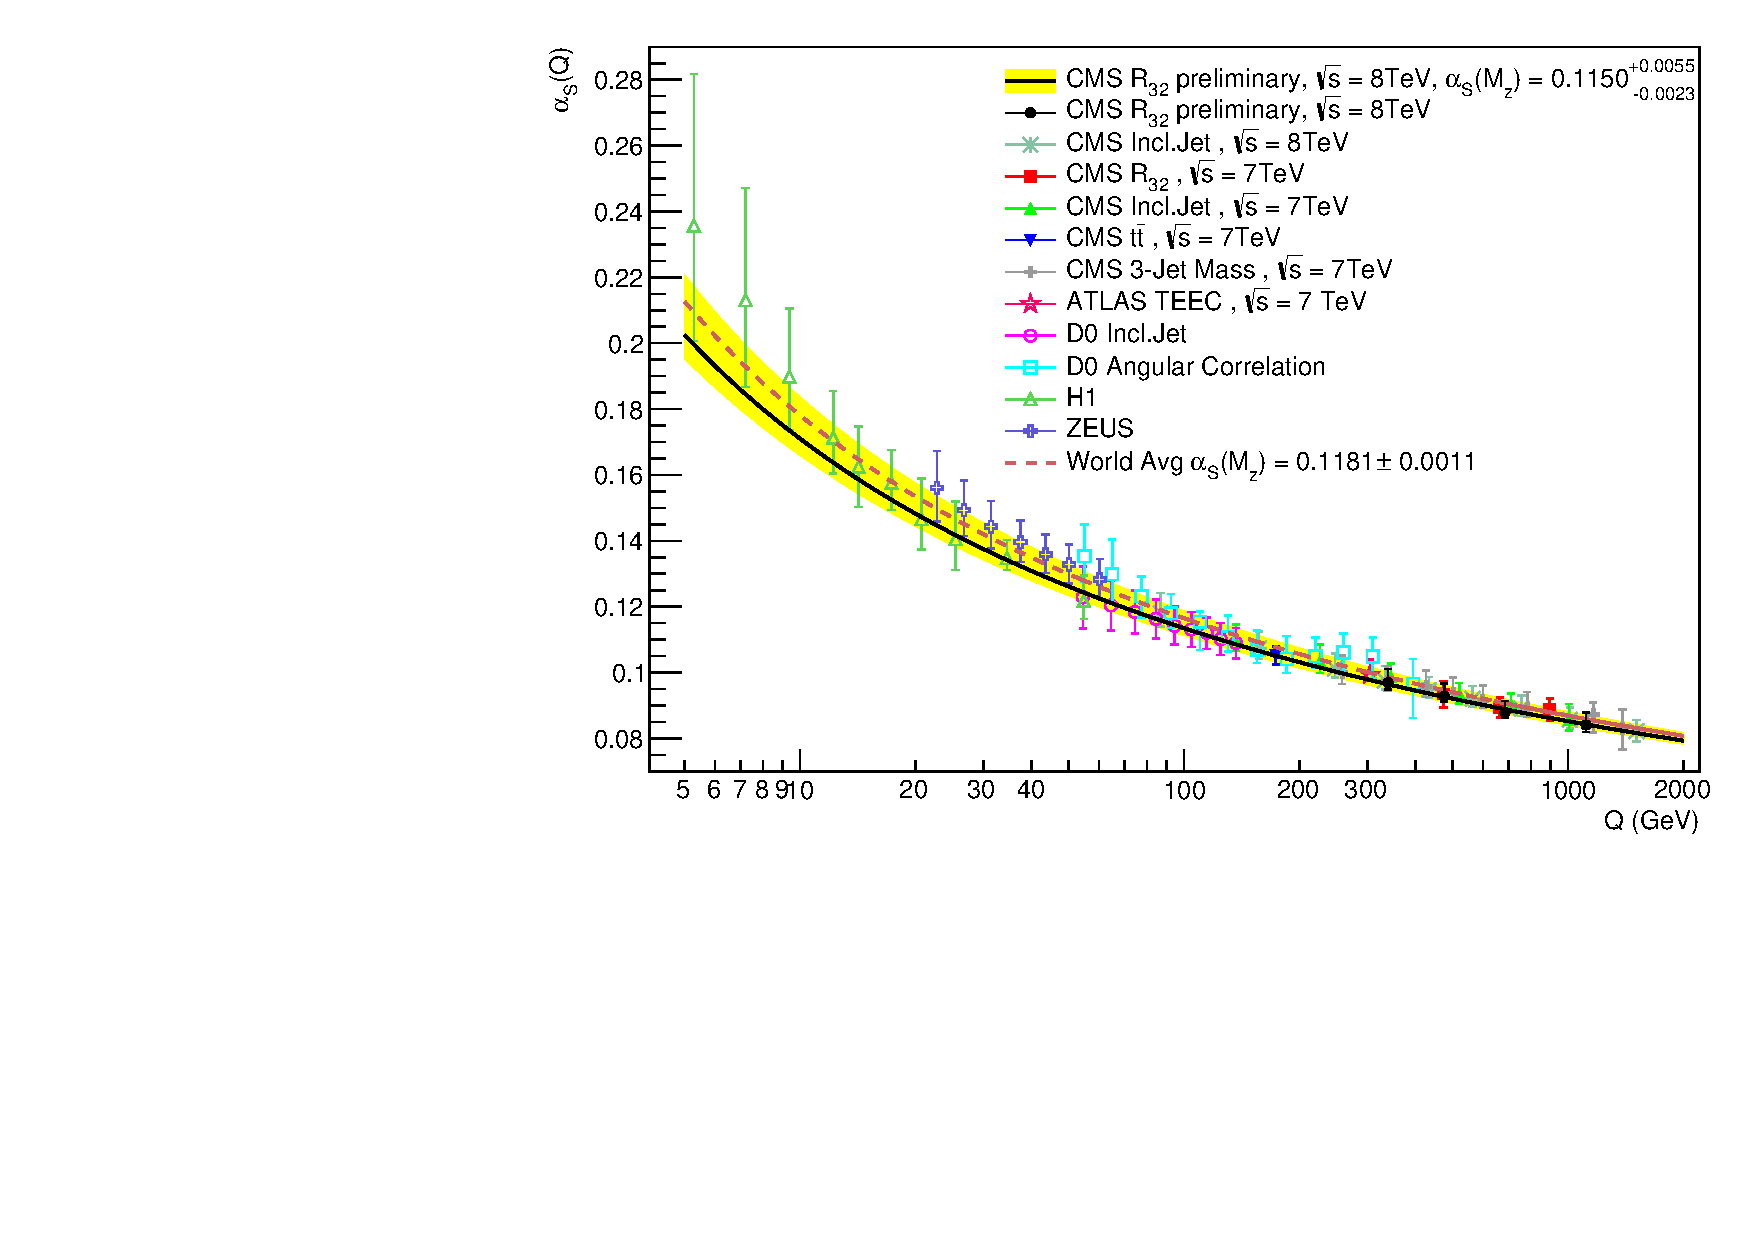
\includegraphics[width=1.05\textwidth]{Plots_HT_2_150/Running_alphas_8TeV_R32.pdf}
 \caption{The running \alpsq as a function of the scale Q is shown as obtained by using the MSTW2008 NLO PDF set. The solid line and the uncertainty band are drawn by evolving the extracted \alpsmz values using the 2-loop 5-flavour renormalization group equations as implemented in \RunDec~\cite{Chetyrkin:2000yt,Schmidt:2012az}. The dashed line represents the evolution of the world average~\cite{Patrignani:2016xqp} and the black circles correspond to the \alpsq determinations presented in Table~\ref{tab:asq_values}. Results from other measurements of CMS~\cite{Chatrchyan:2013txa, Chatrchyan:2013haa, Khachatryan:2014waa, CMS:2014mna, Khachatryan:2016mlc}, ATLAS~\cite{ATLAS:2015yaa}, D0~\cite{Abazov:2009nc, Abazov:2012lua}, H1~\cite{Andreev:2014wwa, Andreev:2016tgi}, and ZEUS~\cite{Abramowicz:2012jz} are superimposed.}
 \label{fig:running_alphas}
\end{figure}
